%\documentclass[11pt,a4paper]{report}
\documentclass[11pt,a4paper]{article}
%\documentclass[11pt,a4paper]{amsart}

% 1 inch margins
\usepackage{fullpage}
\usepackage{framed}
\usepackage{listings}
  \usepackage{courier}
\usepackage{amsmath}
\usepackage{verbatim}
\usepackage{graphicx}             % latex, eps
%\usepackage[pdftex]{graphicx}    % pdflatex, png, jpg, pdf
\usepackage[dvips,usenames,dvipsnames]{color}   % dvips here screws up graphicx png version, above
\usepackage[dvipdf]{hyperref}
%\usepackage{titletoc}
\usepackage{tocloft}

% prevent double digit sub-sections crowding the toc line
\addtolength\cftsubsecnumwidth{0.5em}  % see tocloft manual

\definecolor{codeblock}{rgb}{0.95,0.98,1.0}
%\definecolor{keywords}{rgb}{1.0,0.3,0.0}
\definecolor{keywords}{rgb}{1.0,0.1,1.0}
%\definecolor{comments}{rgb}{0.0,0.7,0.8}
\definecolor{comments}{rgb}{1.0,0.0,0.0}
\definecolor{identifiers}{rgb}{0.1,0.0,1.0}
\definecolor{strings}{rgb}{0.0,0.6,0.0}
\definecolor{basic}{rgb}{0.0,0.4,0.0}

\definecolor{shadecolor}{rgb}{0.9,0.9,0.1}

\lstset{
language=,
%xleftmargin=2em,
%frame=single,
backgroundcolor=\color{codeblock},
basicstyle=\color{basic}\footnotesize\ttfamily,
identifierstyle=\color{identifiers},
keywordstyle=\color{keywords},
commentstyle=\color{comments},
stringstyle=\color{strings},
showstringspaces=false,
%numbers=left,
%numberstyle=\color{Gray}
}

\lstset{
language=bash,
numbers=left,
}

\lstdefinelanguage{cylctaskdef}
{
morekeywords={NAME,DESCRIPTION,TYPE,CONTACT_DELAY,OWNER,CYCLES,TASK,ENVIRONMENT,ESTIMATED_RUN_TIME,PREREQUISITES,STARTUP_PREREQUISITES,OUTPUTS,ESTIMATED_RESTART_OUTPUT_TIMES,NO_NONCOTEMPORAL_DEPENDANTS,ONEOFF_FOLLOW_ON},
sensitive=false,
morecomment=[l]{\#},
morestring=[b]\",
numbers=left,
}

\lstdefinelanguage{usage}
{
%morekeywords={configure, register, unregister, start, pause, resume, stop, insert, reset, kill, purge, task-dump, what-is, run-task, message, set-level, nudge, monitor },
string=[b]{"},
sensitive=false,
morecomment=[l]{Usage:},
morecomment=[l]{USAGE:},
morecomment=[l]{Arguments:},
morecomment=[l]{Options:},
morecomment=[l]{Commands:},
morecomment=[l]{usage:},
morecomment=[l]{arguments:},
morecomment=[l]{command-options:},
morecomment=[l]{COMMANDS:},
morecomment=[l]{options:},
morecomment=[l]{\#}
}

\title{Cylc \linebreak A Self-Organising Optimal Multicycle Scheduler \linebreak For Complex Forecasting Systems \linebreak Version -CYLC-VERSION-}

\author{Hilary Oliver, NIWA}

\begin{document}


\maketitle

\pagebreak

\begin{abstract}

    {\em Cylc} (pronounced ``silk'') is an advanced
    metascheduler\footnote{A metascheduler determines when dependent
    jobs are {\em ready} to run, at which point they can be sent to a
    batch queue scheduler. We drop the ``meta'' prefix from here on,
    however, because a metascheduler is also a type of scheduler. The
    term can also refer to a single aggregate view of multiple
    distributed resource managers, but that is not the topic of this
    document.} for cycling environmental forecast suites containing many
    interdependent scientific models and associated data processing
    tasks.\footnote{A {\em task} is any group of processes treated as a
    single entity for scheduling purposes.} Cylc is internally
    self-organising:\footnote{Prior to version 3.0 cylc's suite design
    interface reflected this too - a suite was defined solely by a set
    of distinct ``task definition files'' that just specified inputs and
    outputs; now, however, one specifies the suite dependency graph up
    front.} its novel scheduling algorithm allows an evolving pool of
    task proxy objects to resolve dependencies amongst themselves so
    that correct scheduling emerges naturally at run time.  Cylc does
    not group tasks artificially by forecast cycle,\footnote{For our
    purposes a {\em forecast cycle} comprises all tasks with a common
    {\em cycle time}, i.e.\ the analysis time or nominal start time of a
    forecast model, or that of the forecast model(s) associated with the
    other tasks.} and its task proxies are individually self-spawning
    (i.e.\ there is no ``global suite forecast cycle'') so that tasks
    from multiple forecast cycles can run at once to the full extent
    allowed by the real inter- and intra-cycle dependencies. This
    matters in particular whenever the external driving
    data\footnote{Forecast systems are typically driven by observational
    data and/or timely model fields from an external forecasting
    system.} for upcoming cycles are available in advance: cylc suites
    can catch up from delays very quickly, parallel test suites can be
    started or restarted behind the main operation to catch up quickly,
    and one can likewise achieve much greater throughput in historical
    case studies. The usual sequence of distinct forecast cycles emerges
    naturally as a suite catches up to real time operation.  Cylc is
    easily interfaced to existing tasks and is extremely flexible.
    Suites can be stopped and restarted in any state of operation, and
    they dynamically adapt to insertion and removal of tasks, and to
    delays or failures in particular tasks or in the external
    environment: tasks not directly affected will carry on cycling as
    normal while the problem is addressed, after which time the affected
    tasks will catch up as quickly as possible. Cylc's handling of
    forecast model restart dependencies, and ability to
    recursively remove entire sub-trees of tasks, allows continued
    operation, with very little intervention, over major failures that
    require omitted forecasts in the driving models. Cylc suites can be
    distributed across a heterogenous network. Cylc has comprehensive
    graphical and command line interfaces, and many advanced userspace
    features: job databases, simulation mode, suite validation,
    dependency graph plotting, centralised alert hooks for failures and
    timeouts, cryptographically secure suites, \ldots

    %\footnote{Cylc also
    %enables new modes of real time operation, for example a catchment
    %river model that runs hourly assimilating real time stream flow
    %observations and using the {\em most recent} 6-hourly precipitation
    %forecast - see EcoConnect, below).} 
\end{abstract}




\pagebreak
\tableofcontents
\listoffigures
%\listoftables

\pagebreak
\section{How Cylc Works} 
\label{HowCylcWorks}

\subsection{Scheduling Forecast Systems} 
\label{SchedulingForecastSystems}

Environmental forecasting systems generate forecast products at regular
intervals using potentially large sets of scientific models and
associated data processing tasks. They are constrained by availability
of external driving data, typically real time observations and/or model
data from an external forecasting system, which one or more tasks depend
on, and these drive other ``downstream'' tasks, and so on. The
dependency diagram for a single forecast cycle in such a system 
is a {\em Directed Acyclic Graph} (a {\em forecast cycle} is comprised
of tasks with a common {\em cycle time}, namely the nominal analysis
time or start time of the forecast models in the group). Normal real
time operation necessarily consists of a series of distinct forecast
cycles that are each initiated, after a gap in processing, by arrival of
new external driving data.

From a job scheduling perspective task execution order must be carefully
controlled in order to avoid dependency violations. Ideally, each task
should be queued for execution at the instant its last prerequisite is
satisfied; this is the best that can be done even if queued tasks are
not able to execute immediately because of resource contention.


\subsection{EcoConnect} 
\label{EcoConnect}

This work was motivated by the EcoConnect Forecasting System at NIWA
(National Institute of Water and Atmospheric Research, New Zealand). As
of 2009, EcoConnect takes real time atmospheric and stream flow
observations, and operational global weather forecasts from the Met
Office (UK), and uses these to drive global sea state and regional data
assimilating weather models, which in turn drive regional sea state,
storm surge, and catchment river models, plus tide prediction, and a
large number of associated data collection, quality control,
preprocessing, postprocessing, product generation, and archiving
tasks.\footnote{Future plans for EcoConnect include additional
deterministic regional weather forecasts and a statistical ensemble.}
The global sea state forecast runs once daily.  The regional weather
forecast runs four times daily but it supplies surface winds and
pressure to several downstream models that run only twice daily, and
precipitation accumulations to catchment river models that run on an
hourly cycle assimilating real time stream flow observations and using
the most recent available regional weather forecast.  EcoConnect runs on
heterogenous distributed hardware, including a massively parallel
supercomputer and several Linux servers. 

\subsection{Intracycle Dependencies} 
\label{IntracycleDependencies}

Because real time operation consists of a series of distinct forecast
cycles, it is natural to consider dependencies that occur between tasks
within a single forecast cycle. A sea state forecast, for example, might
depend on surface wind fields generated by a weather forecast over the
same forecast range, and a postprocessing task clearly cannot run before
its input data has been generated. Figure~\ref{fig-dep-one} shows the
dependency diagram for a single forecast cycle of a simple example
system consisting of three forecast models ({\em a, b,} and {\em c}) and
three post processing or product generation tasks ({\em d, e} and {\em
f}).  A scheduler capable of handling this must manage, within a single
forecast cycle, multiple parallel streams of execution that branch when
one task generates output for several downstream tasks, and merge when
one task takes input from several upstream tasks. 

\begin{figure} \label{fig-dep-one} 
    \begin{center}
        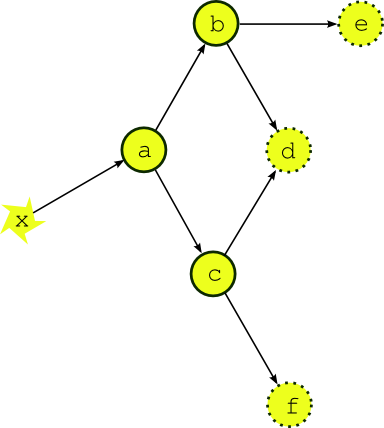
\includegraphics[width=6cm]{inkscape-svg/dep-one-cycle} 
    \end{center}
    \caption[Single cycle dependency graph for a simple system]{\small
    The dependency graph for a single forecast cycle of a simple example
    system. Tasks {\em a, b,} and {\em c} represent forecast models,
    {\em d, e} and {\em f} are post processing or product generation
    tasks, and {\em x} represents external data that the upstream
    forecast model depends on.}
\end{figure} 

\begin{figure} \label{fig-time-one}
    \begin{center}
        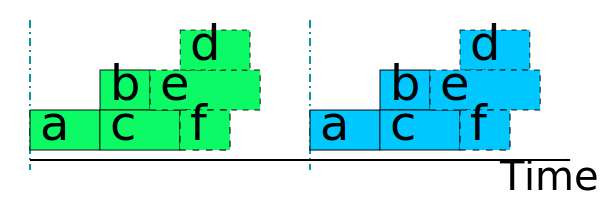
\includegraphics[width=8cm]{inkscape-svg/timeline-one}
    \end{center}
    \caption[Single cycle job schedules for real time operation]{\small
    The optimal job schedule for two consecutive cycles of our example
    system during real time operation, assuming that all tasks trigger 
    off upstream tasks finishing completely. The horizontal extent of
    a task bar represents its execution time, and the vertical blue
    lines show when the external driving data becomes available.}
\end{figure}

Figure~\ref{fig-time-one} shows the optimal job schedule for two
consecutive cycles of the example system in real time operation, given
execution times represented by the horizontal extent of the task bars.
There is a time gap between cycles as the system waits on new external
driving data.  Each task in the example system happens to trigger off
upstream tasks {\em finishing}, rather than off any intermediate output
or event; this is merely a simplification to make for clearer diagrams.

\begin{figure} \label{fig-dep-two-linked}
    \begin{center}
        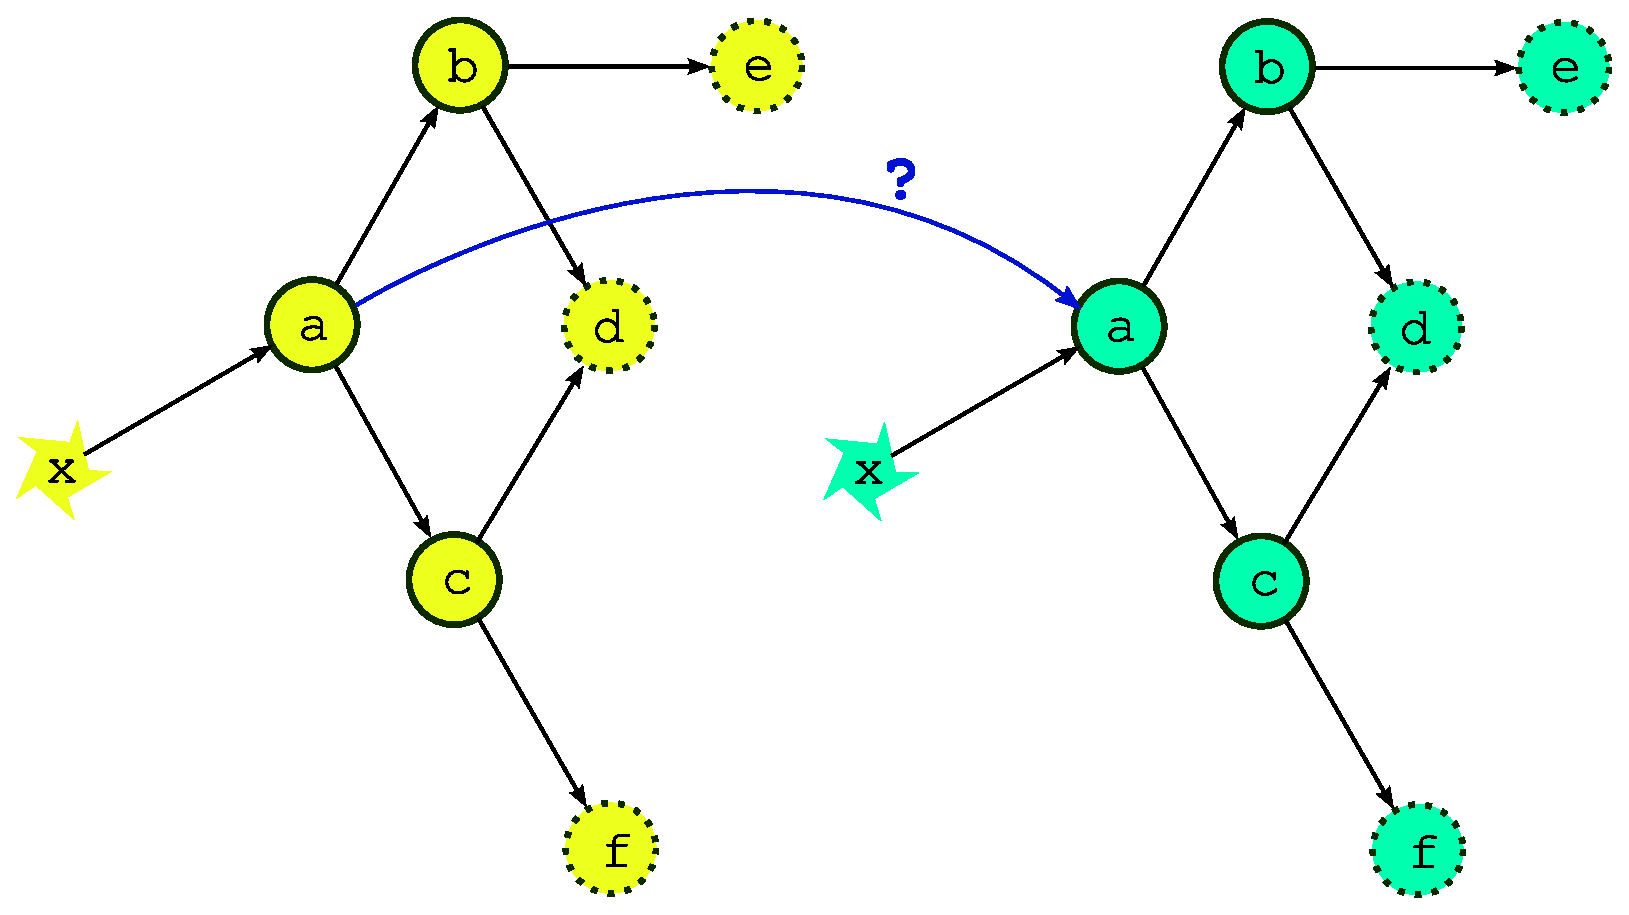
\includegraphics[width=10cm]{inkscape-svg/dep-two-cycles-linked} 
    \end{center}
    \caption[What if the external data is available early?]{\small If
    the external driving data is available in advance, can we start
    running the next cycle early?} 
\end{figure}

\begin{figure} \label{fig-overlap}
    \begin{center}
        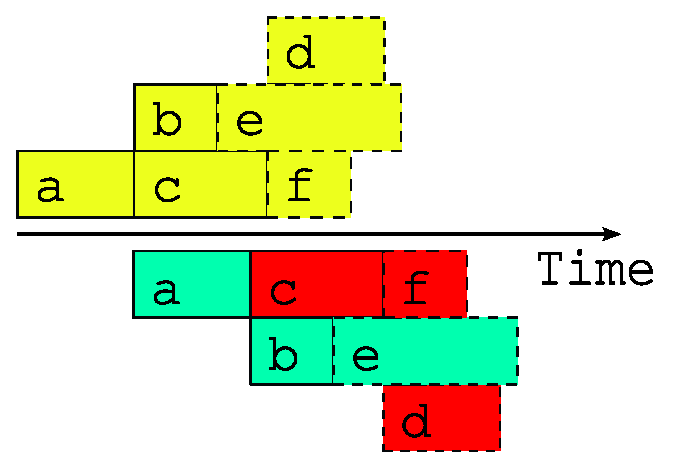
\includegraphics[width=6cm]{inkscape-svg/timeline-one-c} 
    \end{center}
    \caption[Attempted overlap of consective single-cycle job
    schedules]{\small A naive attempt to overlap two consecutive cycles
    using the single-cycle dependency graph. The red shaded tasks will
    fail because of dependency violations (or will not be able to run
    because of upstream dependency violations).} 
\end{figure} 

\begin{figure} \label{fig-job-no-overlap}
    \begin{center}
        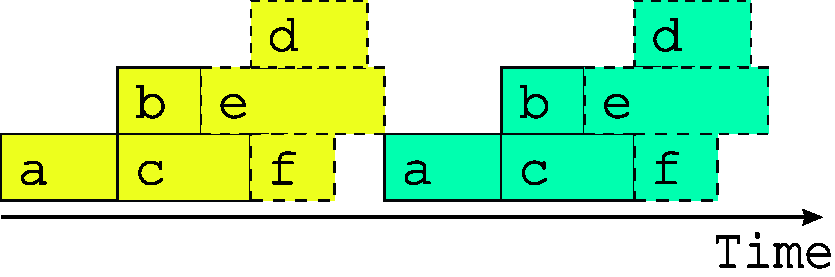
\includegraphics[width=8cm]{inkscape-svg/timeline-one-a} 
    \end{center}
    \caption[The only safe multicycle job schedule?]{\small The best that
    can be done {\em in general} when intercycle dependencies are
    ignored.} 
\end{figure} 

Now the question arises, what happens if the external driving data for
upcoming cycles is available in advance, as it would be after a
significant delay in operations, or when running a historical case
study?  The forecast model {\em a} depends only on the external data
and, implicitly at this stage of the discussion, on its own previous
instance for a model ``background state''. Thus, as alluded to in
Figure~\ref{fig-dep-two-linked}, task {\em a} could in principle start
immediately its predecessor has finished.  Figure~\ref{fig-job-two}
shows, however, that starting a whole new cycle at this point is
dangerous - it results in dependency violations in half the tasks of the
simple example system. In fact the situation is even worse than this -
what if task {\em b} in the first cycle is delayed for any reason {\em
after} the second cycle has been launched? Clearly we must consider
handling intercycle dependencies explicitly in order to solve this
problem, or else agree never to start the next cycle early as
is illustrated in Figure~\ref{fig-job-no-overlap}.


\subsection{Intercycle Dependencies} 
\label{IntercycleDependencies}

In any non-trivial system dependencies between tasks in different cycles
exist. Forecast models typically depend on their own most recent
previous forecast for an initial ``background state'', and different
types of tasks in different forecast cycles can also be linked (e.g.\
the complicated relationship between the weather and river models in
EcoConnect). {\em In real time operation these intercycle dependencies
can be ignored because they are automatically satisfied when each cycle
necessarily finishes before the next one begins.} This is just as well
because they dramatically increase the complexity of the dependency
graph of even the simplest systems, by destroying the clean boundary
between forecast cycles. Figure~\ref{fig-dep-multi} illustrates the
problem for our simple example system assuming the minimal likely
intercycle dependence: the forecast models ($a$, $b$, and $c$) each
depend on their own previous instances.

For this reason, and because we tend to see forecasting systems as
running in distinct cycles, all existing schedulers (as far as the
author is aware!) ignore intercycle dependencies and therefore require a
series of distinct cycles at all times. While this does not affect
normal real time operation it can be a serious impediment when advance
availability of external driving data makes it possible, in principle,
to run some tasks from upcoming cycles before the current cycle is
finished - as suggested at the end of the previous section. This occurs
after delays (late arrival of external data, system maintenance, etc.)
and, to an even greater extent, in historical case studies, and parallel
test systems that are delayed with respect to the main operation. It is
a serious problem, in particular, for systems that have little downtime
between forecast cycles and therefore take many cycles to catch up
after a delay. Without taking account of intercycle dependencies, the
best that can be done, in general, is to reduce the gap between cycles
to zero as shown in Figure~\ref{fig-job-no-overlap}. A limited crude
overlap of the single cycle job schedule may be possible for specific
task sets, but it must be borne in mind that this may change if new
tasks are added, and it amounts to running different parts of a
dependant system as if they were not dependant; as such it cannot be
guaranteed that unforeseen delays in one cycle won't result in
dependency violations in the next.

\begin{figure} \label{fig-dep-multi}
    \begin{center}
        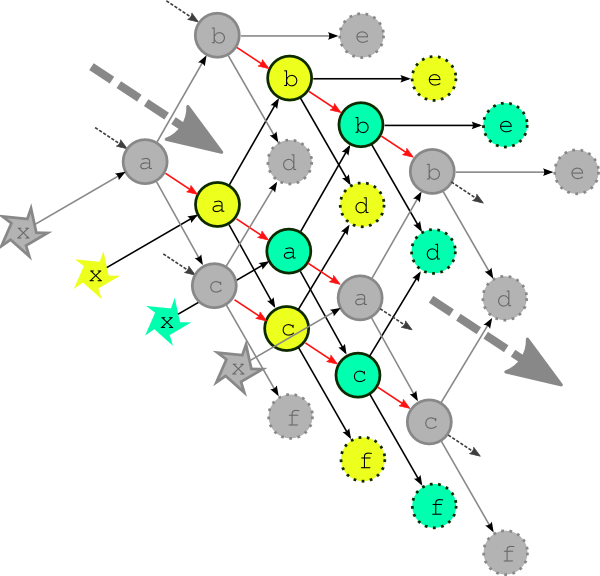
\includegraphics[width=8cm]{inkscape-svg/dep-multi-cycle} 
    \end{center}
    \caption[Complete multicycle dependency graph]{\small The complete
    dependency graph for the example system, assuming the least possible
    intercycle dependence: the forecast models ($a$, $b$, and $c$)
    depend on their own previous instances. The dashed arrows show
    connections to previous and subsequent forecast cycles.} 
\end{figure}

\begin{figure} \label{fig-optimal-two}
    \begin{center}
        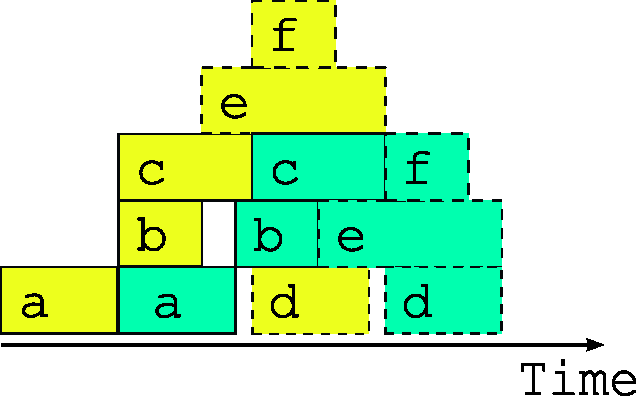
\includegraphics[width=6cm]{inkscape-svg/timeline-two-cycles-optimal} 
    \end{center}
    \caption[Optimal two-cycle job schedule]{\small Optimal two cycle
    job schedule when the next cycle's driving data is available in
    advance, possible in principle when intercycle dependencies are
    handled explicitly.} 
\end{figure} 

Figure~\ref{fig-optimal-two} shows, in contrast to
Figure~\ref{fig-overlap}, the optimal two cycle job schedule obtained by
respecting all intercycle dependencies. It must be noted, however, that
this job schedule assumes ideal conditions with no delays due to
resource contention or anything else - i.e.\ every task is able to run
in its alotted time as soon as it is ready to run. The scheduler running
this system must be able to adapt dynamically to external conditions 
that impact on multicycle scheduling in the presence of
intercycle dependencies or else, again, risk bringing the system down
with dependency violations.

\begin{figure} \label{fig-time-three}
    \begin{center}
        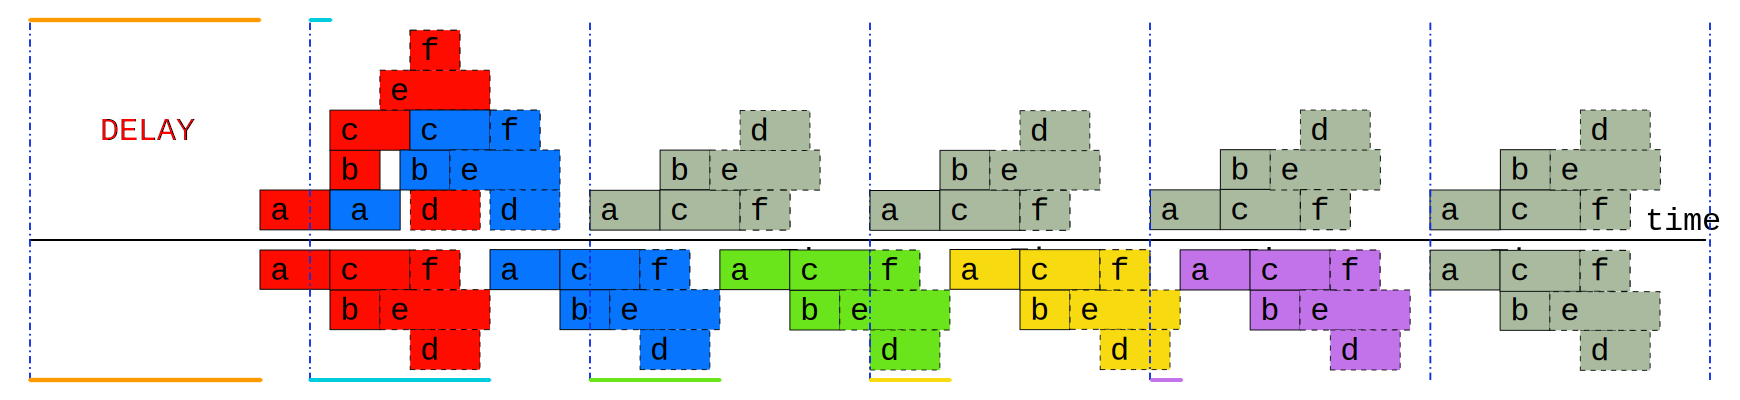
\includegraphics[width=12cm]{inkscape-svg/timeline-three} 
    \end{center}
    \caption[Post delay comparison of job schedules]{\small Job
    schedules for the example system after a delay of almost one whole
    forecast cycle, when intercycle dependencies are
    taken into account (above the time axis), and when they are not
    (below the time axis). The colored lines indicate the time that
    each cycle is delayed, and normal ``caught up'' cycles
    are shaded gray.} 
\end{figure} 

\begin{figure} \label{fig-time-two}
    \begin{center} 
        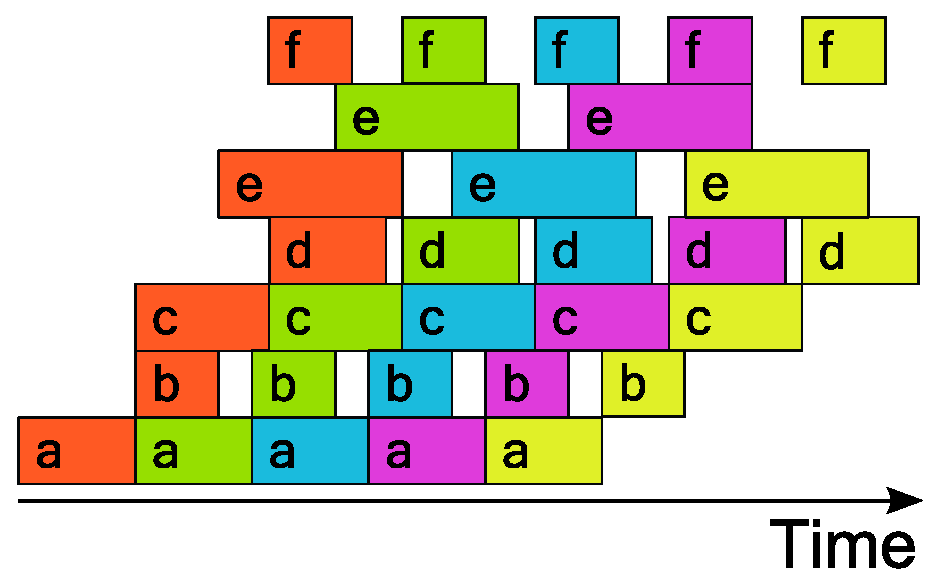
\includegraphics[width=8cm]{inkscape-svg/timeline-two}
    \end{center} 
    \caption[Optimal job schedule when all external data is
    available]{\small Job schedules for the example system in case study
    mode, or after a long delay, when the external driving data are
    available many cycles in advance. Above the time axis is the optimal
    schedule obtained when the system is constrained only by its true
    dependencies, as in Figure \ref{fig-dep-two}, and underneath is
    the best that can be done, in general, when intercycle dependencies
    are ignored.} 
\end{figure} 

To further illustrate the potential benefits of proper intercycle
dependency handling, Figure~\ref{fig-time-three} shows an operational
delay of almost one whole cycle in a system with little downtime between
cycles. Above the time axis is the optimal schedule that is possible, in
principle, when intercycle dependencies are taken into account, and
below is the only safe schedule possible {\em in general} when they are
ignored.  In the former case, even the cycle immediately after the delay
is hardly affected, and subsequent cycles are all on time, whilst in the
latter case it takes five cycles to catch up again to normal real time
operation. Note that simply overlapping the single cycle schedules of
Figure~\ref{fig-time-one} from the same start point would have resulted
in dependency violation by task {\em c}.

Similarly, Figure~\ref{fig-time-two} shows example system job schedules
for an historical case study, or when catching up after a very long
delay; i.e.\ when the external driving data are available many cycles in
advance.  Task {\em a}, which as the most upstream forecast model is
likely to be a resource intensive atmosphere or ocean model, has no
dependence on cotemporal tasks and can therefore run continuously,
regardless of how much downstream processing is yet to be completed in
its own, or any previous, forecast cycle. In practice task {\em a} would
depend on cotemporal upstream tasks that wait on the external driving
data, but they would return immediately when the external data is
available in advance, so the result stands. The other forecast models
can also cycle continuously or with short gap between, and some post
processing tasks, which have no previous-instance dependence, can also
run continuously or even overlap (e.g.\ {\em e} in this case).  Thus,
even for this very simple example system, tasks from three or four
different cycles can in principle run simultaneously at any given time. 

Finally we note again the additional obstacles in the way of achieving
this optimal multicycle job scheduling. Firstly, the scheduler must be
able to dynamically adapt to delays due to resource contention, varying
run times, or whatever, which will result in non-trivial changes to
these already non-trivial job schedules. Secondly, given advance
availablility of the external input data and any other inputs supplied
by other models, forecast models can in principle start well {\em
before} their previous instance has finished (because restart outputs
for the next cycle are generated early in a forecast run). And
similarly, but more generally, we may well want some tasks to trigger
off intermediate upstream outputs rather than waiting for upstream tasks
finish entirely. 


\subsection{The Cylc Scheduling Algorithm} 
\label{TheCylcSchedulingAlgorithm}

\begin{figure} \label{fig-task-pool}
    \begin{center} 
        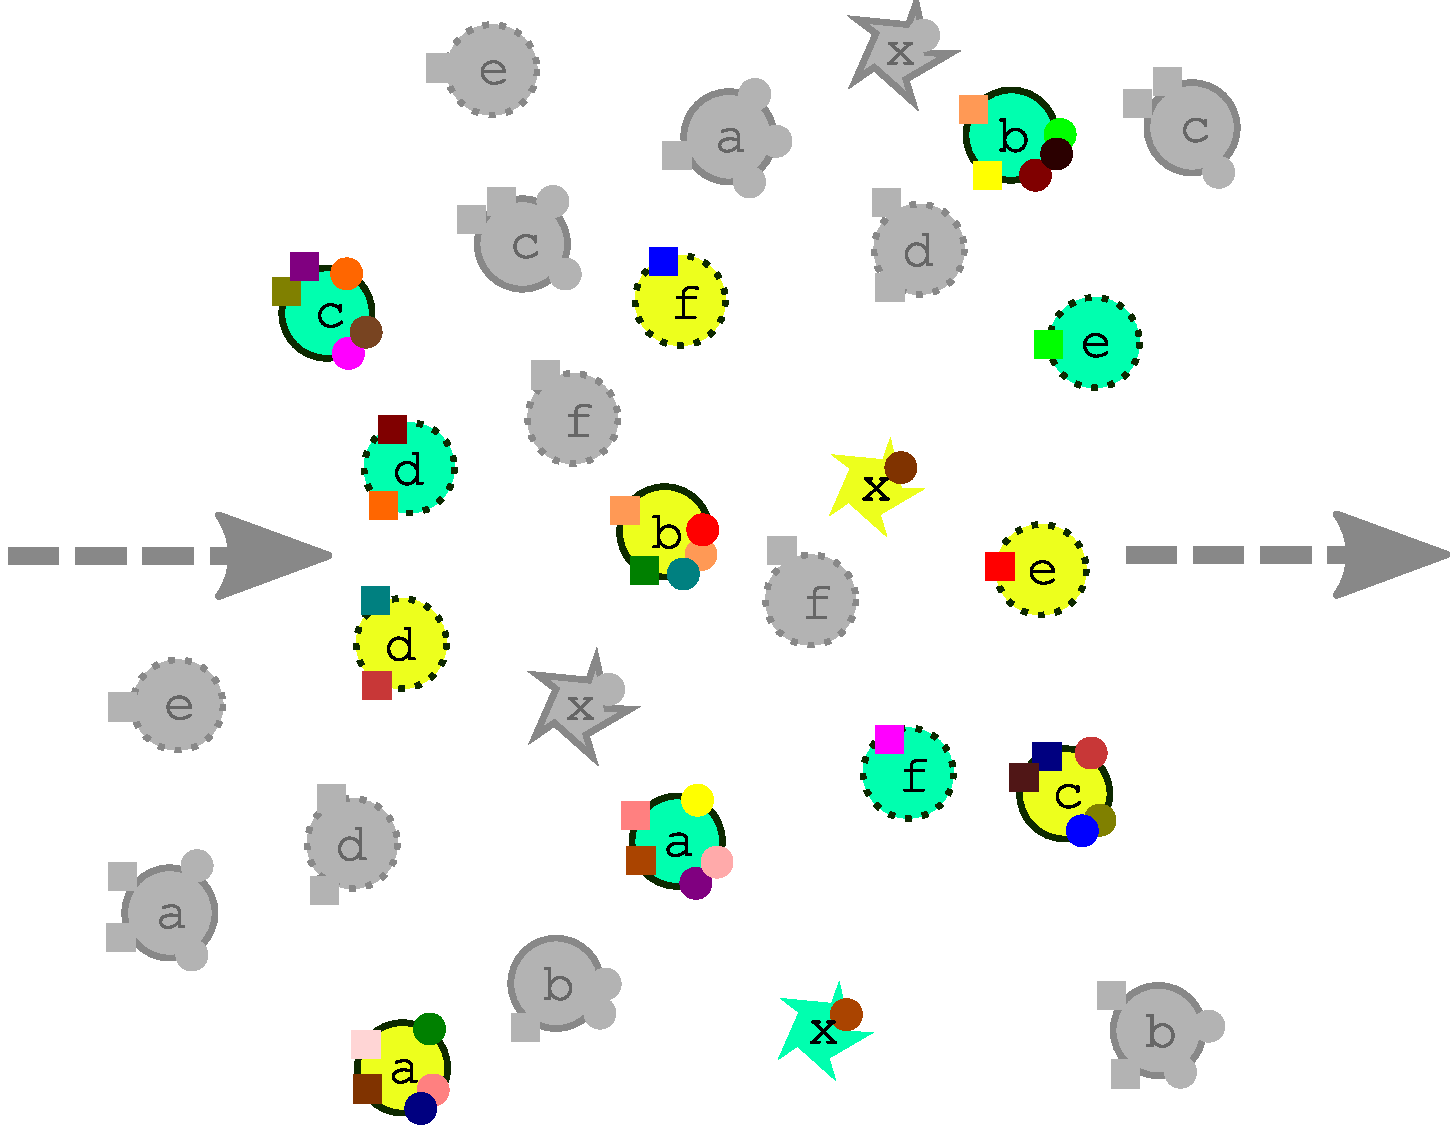
\includegraphics[width=8cm]{inkscape-svg/task-pool}
    \end{center} 
    \caption[The cylc task pool]{\small How cylc sees the task pool, in
    contrast to the full dependency diagram of Figure~\ref{fig-full}.} 
\end{figure} 

This section explains how cylc achieves the optimal multicycle
scheduling described above. 

Cylc manages a pool of proxy objects that represent real tasks in the
forecasting system. A task proxy object can run the real task when its
prerequisites are satisfied, and can receive reports of completed
outputs from the real task as it runs. There is no global cycling
mechanism to advance the system in time; instead each individual task
proxy has a private cycle time and spawns its own successor at the right
time (which depends only on the task's own type and state). Task proxies
are self-contained and do not know what other tasks exist in the system,
they just know their own prerequisites and outputs.  Prerequisites can
equally represent intra- and intercycle dependencies, and the task pool
can be populated with tasks having many different cycles. Now,
whenever any task proxy changes state (as a result of an output
completion message, for example) cylc gets the entire pool to interact
indiscriminately, {\em regardless of cycle times}, in an attempt to
match unsatisfied prerequisites with completed outputs.\footnote{In fact
this dependency negotiation goes through a middleman or broker object,
which reduces the interaction scaling from $n^2$ to $n$, where $n$ is
the number of task proxies.} 

Thus without using global cycling mechanisms, and treating all
dependencies equally, cylc in effect gets a set of individual tasks to
self-organise by negotiating their own dependencies: optimal scheduling,
as illustrated in the previous section, emerges naturally at run time.

In addition, cylc makes no distinction between delayed and real time
operation. In delayed operation the tasks that gather the system's
external driving data will return immediately (because the data is
already available) and the system will only be constrained by its
internal dependencies. In real time operation, the data gathering tasks
will return only when the external data becomes available (normally at
some known time interval after the task's nominal cycle time), delaying
downstream tasks until then, by which time the previous forecast cycle
will have completed. A cylc system thus transitions seamlessly from
optimal multicycle scheduling to ``normal'' distinct forecast cycles as
it catches up to real time operation.

Note that in addition to achieving optimal scheduling, this algorithm is
extremely simple. The operator does not have to construct a special
``suite'' in which order of execution or explicit dependency
relationships are specified (except implicitly, in that each task's
prerequisites must be matched by someone's outputs). Instead the entire
forecasting system is defined by a simple list of tasks each of which,
in effect, thinks it is alone in the world (even a standalone task must
know its own prerequisites and outputs).

%\footnote{However, you can still use explicit task dependence if you
%wish: just make a task depend on an explicitly named upstream supplier
%{\em finishing} rather than on the upstream output that is the actual
%prerequisite of interest. However, framing prerequisites in terms of
%required input filenames, or similar, results in a more flexible
%system: tasks can easily be ``hot replaced'' by others that generate
%similar outputs.}

Perhaps the most difficult problem encountered during cylc
implementation was how to arrange that every task proxy object exists by
the time it is needed, but not too much earlier, and does not die too
long after it is no longer needed. This engendered no small amount
of hair pulling and teeth gnashing, but once achieved the complexities
therein are entirely hidden from the user.

%In other words the task pool must include waiting tasks whose
%prerequisites may {\em soon} be satisfied (but preferably no waiting
%tasks whose prerequisites will not be satisfied for some time yet),
%tasks that are currently running, and finished tasks whose outputs
%could still be needed by any current or future waiting task (but
%preferably not any finished tasks whose output will no longer be needed
%by anyone). 



\pagebreak

\section{The Cylc Command Set}
\lstset{language=usage}
\lstinputlisting{command-usage/help.txt}
\pagebreak

\section{Installation And Testing} 
\label{InstallationAndTesting}

\subsection{Requirements} 
\label{Requirements}

\begin{itemize}
    \item Unix or Linux
    \item Python
    \item Pyro (Python Remote Objects)
\end{itemize}

Cylc has been tested with Python~2.6, and Pyro~3.9 and 3.10,
but it should work with any recent versions of Python~2 and Pyro.
As yet neither cylc nor Pyro are compatible with Python~3. 

\subsection{Getting Cylc} 
\label{GettingCylc}

See Appendix~\ref{Pyro} for Pyro download directions.

Cylc is currently maintained using {\em darcs} (http://darcs.net), a
distributed revision control system. If you need to develop cylc you can
request access to clone the central repository, otherwise you will
receive a cylc release tarball. 

\subsection{Installation} 
\label{Installation}

Pyro installs easily into the standard Python modules path on your
system; follow Pyro's own installation instructions.

Cylc is designed to be installed into a normal user account: simply
unpack the tarball, or move the repository, to the location of your
choice. There is no ``build'' required because cylc is written in Python
(plus a few small bash scripts).

\subsection{Environment} 
\label{Environment}

\lstset{language=bash} 

The cylc bin directory must be in your executable search path, to
provide access to cylc commands, and the cylc source directory must be
in your Python module search path, to provide access to the cylc core
modules. To configure your current command shell for cylc, source 
the environment script \lstinline=cylc-env.sh= from the directory it
resides in (i.e.\ the top level of your cylc installation):

\begin{lstlisting}
$ . cylc-env.sh
\end{lstlisting}

Or for automatic access, put the following in your (sh-style) login
script:

\begin{lstlisting}
# CYLC
export CYLC_DIR=$HOME/cylc  # (the install location)
. $CYLC_DIR/cylc-env.sh
\end{lstlisting}


\subsection{Testing} 
\label{Testing}

Test the new installation by running the packaged ``userguide'' example
system, and compare the results with the scheduling diagrams in
Section~\ref{TheCylcSchedulingAlgorithm}. The packaged examples should
work ``out of the box'' in real and dummy mode, using the simple
sequence of commands presented in the Quick Start Guide, from {\em
Prepare For Scheduling} (Section~\ref{QuickPrepareForScheduling})
onward.  For detailed information on the packaged example systems, refer
to {\em A Complete Working Example}
(Section~\ref{ACompleteWorkingExample}).  

\pagebreak
\section{Quick Start Guide} 
\label{QuickStartGuide}

\lstset{language=bash}

This section is intended as a quick introduction to, or reminder of,
basic cylc functionality. The specific commandline listings below use
the packaged cylc ``userguide'' example system. Refer to 
\lstinline=cylc help=, the {\em Command Reference}
(Section~\ref{CommandReference}), and
upcoming sections of this document for more detailed information on
available commands, options, and operations.  {\em A Complete Working
Example} (Section~\ref{ref:ACompleteWorkingExample} describes the
userguide example system in detail.

\subsection{Starting A Pyro Nameserver}
\label{QuickStartingAPyroNameserver}

Pyro (Appendix~\ref{Pyro}) is the object oriented Python RPC framework
that allows system tasks to communicate with their proxy objects inside
a cylc scheduler. First check to see if there is already a Pyro
nameserver (\lstinline=pyro-ns=) running on your network segment:

\begin{lstlisting}
# search for a Pyro nameserver on the network
$ pyro-nsc ping
Locator: searching Pyro Name Server...
Locator: retry 1
Locator: searching Pyro Name Server...
Locator: retry 1
Trying host oliverh-33191VL
Locator: contacting Pyro Name Server...
NS is at 127.0.0.2 (oliverh-33191VL.greta.niwa.co.nz) port 9090
NS is up and running!

# search for a Pyro nameserver on a specific host
$ pyro-nsc -h localhost ping
Locator: contacting Pyro Name Server...
NS is at 127.0.0.1 (localhost) port 9090
NS is up and running!
\end{lstlisting}

If not, start one up as follows:

\begin{lstlisting}
# start a Pyro nameserver
$ pyro-ns
*** Pyro Name Server ***
Name server listening on: ('0.0.0.0', 9090)
Broadcast server listening on: ('255.255.255.255', 9090)
URI is: PYRO://192.168.56.146:9090/c0a838921e021d8a88b563c085c323e5f4
URI written to: /home/oliverh/Pyro_NS_URI
Name Server started.
\end{lstlisting}

Note that you can start the nameserver with the \lstinline=nohup=
command (\lstinline=man nohup=) to it from dying when your terminal
session logs out.

\subsection{Defining A Task Set} 
\label{QuickDefiningATaskSet}

Before you can run a forecast system with cylc, you need to define the
interface between the scheduler and your real system tasks.  This
is covered in detail in {\em System Definition}
(Section~\ref{SystemDefinition}), but in summary it requires:

\begin{itemize}
    \item defining {\em prerequisites} and {\em outputs} for each task.

    \item writing a simple {\em task definition file} for each task.

    \item ensuring that each task reports its outputs using cylc's
        messaging mechanism.  This may involve writing new {\em task
        scripts}, or slightly modifying existing task execution scripts,
        or using cylc's automatic {\em task wrapping} mechanism
        (Section~\ref{TaskWrapping}) to run unmodified existing tasks.
\end{itemize}


\subsection{Preparing For Scheduling}
\label{QuickPreparingForScheduling}

\subsubsection{System Configuration}
\label{QuickConfiguration}

The configuration process (Section~\ref{SystemConfiguration}) generates
system-specific Python modules in the system definition directory. This
must be done initially, and thereafter whenever the system's task
definition files have been changed:

\begin{lstlisting}
cylc configure $CYLC_DIR/systems/userguide
\end{lstlisting}

\subsubsection{System Registration}
\label{QuickRegistration}

System registration (Section~\ref{SystemRegistration}) associates a name
with a configured system, for a particular user. This is required in
order to {\em run} a system but you can monitor or otherwise interact
with running systems that have been registered and started up by other
users.

\begin{lstlisting}
cylc register --system=$CYLC_DIR/systems/userguide userguide 
\end{lstlisting}

To see your current system registrations, use 
\lstinline=cylc register --print=.

\subsection{Starting The Scheduler}
\label{QuickStartingTheScheduler}

To begin scheduling a registered system:
\begin{lstlisting}
cylc start --at=2009082312 userguide
\end{lstlisting}

In real mode (as opposed to {\em dummy mode}, Section~\ref{DummyMode})
{\em do not choose a start time in the future}, or nothing will happen
until the start time comes up!

You can run multiple systems at once, even multiple instances of the
same system (so long as it is registered under multiple names, and the
external tasks are configured to use the registered name in all input
and output file paths, etc.; the userguide example system is capable of
this). 

\subsection{Following System Progress}
\label{QuickFollowingSystemProgress}

\subsubsection{System Monitors}
\label{QuickSystemMonitors}

\begin{figure} \label{fig-monitor} 
    \begin{center}
        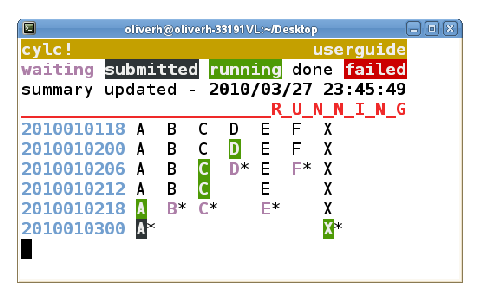
\includegraphics[width=8cm]{monitor-1} 
    \end{center}
    \caption{\small The main terminal-based cylc system monitor}
\end{figure} 

\begin{figure} \label{fig-monitor-r} 
    \begin{center}
        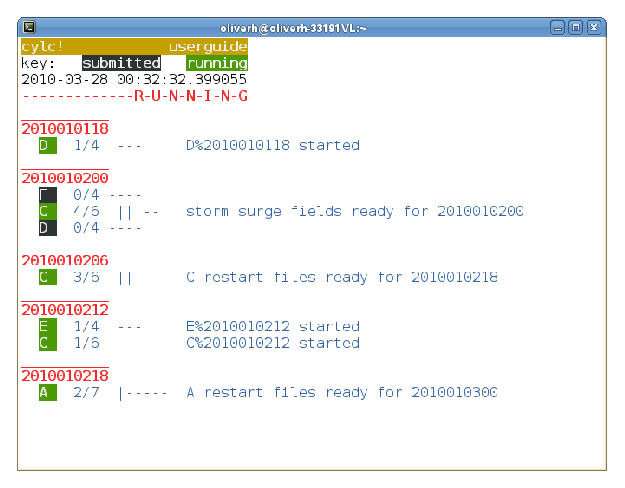
\includegraphics[width=10cm]{monitor-2} 
    \end{center}
    \caption{\small Another terminal-based cylc system monitor}
\end{figure} 


 We currently have just two
terminal-based monitors, which are effective but somewhat primitive.
The standard monitor (Figure~\ref{fig-monitor}) shows the current state
of all task proxy objects in the task pool:

\begin{lstlisting}
# in a new terminal!
cylc monitor --align userguide
\end{lstlisting}

The \lstinline=--align= option causes tasks to be displayed in columns
(which is only useful for small systems in which all task names can fit
on a single line).  Another system monitor (Figure~\ref{fig-monitor-r})
shows the progress of just the running tasks in the pool:

\begin{lstlisting}
# in a new terminal!
cylc monitor-r userguide
\end{lstlisting}

Section~\ref{SystemMonitors} discusses the limitations of the
current system monitors, and plans for future development.

\subsubsection{System Log Files}
\label{QuickSystemLogFiles}

You can also follow system progress in the system log files, which are
discussed in {\em Logging}, Section~\ref{Logging}. By
default these are located under \lstinline=$HOME/cylc-logs/{SYSTEM}=.
Each task has its own log file for task-specific events, including 
incoming task messages, and the \lstinline=main= log file records all
events in sequence.

\lstset{language=,
basicstyle=\color{basic}\scriptsize\ttfamily,
}
\begin{lstlisting}
$ tail $HOME/cylc-logs/userguide/main
2010/03/28 00:33:50 INFO main.F - [2010010312] disconnected (spent; general)
2010/03/28 00:33:52 INFO main.C - [2010010400] storm surge fields ready for 2010010400
2010/03/28 00:33:52 INFO main.A - [2010010412] surface wind fields ready for 2010010412
2010/03/28 00:33:52 INFO main.C - [2010010400] C%2010010400 completed
2010/03/28 00:33:52 INFO main.C - [2010010400] C%2010010400 finished
2010/03/28 00:33:52 INFO main.A - [2010010412] surface pressure field ready for 2010010412
2010/03/28 00:33:52 INFO main.A - [2010010412] level forecast fields ready for 2010010412
2010/03/28 00:33:53 INFO main.A - [2010010412] A%2010010412 completed
2010/03/28 00:33:53 INFO main.A - [2010010412] A%2010010412 finished
2010/03/28 00:33:53 CRITICAL main - ALL RUNNING TASKS FINISHED
\end{lstlisting}

\lstset{language=,
basicstyle=\color{basic}\footnotesize\ttfamily,
}

Each entry shows the time of logging, the name and cycle time of the
reporting task (in square brackets), and the logged message.

\subsubsection{Getting Task State Information}
\label{QuickGettingTaskStateInformation}

To display the current state of a particular task (choose one that
currently exists in the system, according to the monitor):

\begin{lstlisting}
% cylc task-dump -t X%2010010112 userguide
_______________________________
Task X%2010010112 in userguide:
 + => prerequisite satisfied, or output completed
 - => prerequisite NOT satisfied, or output NOT completed
______________
Prerequisites:
(None)
________
Outputs:
 + X%2010010112 completed
 + X%2010010112 finished
 + X%2010010112 started
 + obs data ready for 2010010112
______
Other:
delayed start time reached ... True
\end{lstlisting}

\subsection{Shutting A System Down}
\label{QuickShuttingASystemDown}

\lstset{language=bash}

Before shutting a system down - or indeed using any of the other cylc
commands that can change the state of a running system but are not 
covered in this Quick Start Guide (reset, kill, purge, pause, etc.) -
you need to unlock the system:

\begin{lstlisting}
# unlock:
cylc unlock userguide
# shutdown:
cylc stop userguide
\end{lstlisting}

\subsection{Restarting A System}
\label{QuickRestartingASystem}

You can restart a system from a previous state:

\begin{lstlisting}
cylc start --restart userguide
\end{lstlisting}

Cylc automatically dumps extra time-stamped state files prior to any
system intervention, so that if necessary you can easily restart the
system in its pre-intervention state.  See {\em Restarts}
(Section~\ref{Restarts}) for more information.


\pagebreak
\section{System Definition} 
\label{SystemDefinition}

This section of the userguide explains how to get a system running under
cylc.

%Cylc sees a forecasting system as an evolving, self-organising pool of
%tasks with clearly defined {\em prerequisites} and {\em outputs}, as
%explained in {\em The Cylc Scheduling Algorithm} (Section~\ref{TheCylcSchedulingAlgorithm}). 

First the system must be divided into tasks with clearly defined
prerequisites and outputs (Section~\ref{PrerequisitesAndOutputs}). Then
the properties of each task that are relevant to scheduling must be
declared in {\em cylc task definition files}
(Section~\ref{TaskDefinitionFiles}). Once such property is the script or
executable that should be called to actually execute the real task when
it is ready to run. These {\em task scripts} can be located anywhere,
but if you are creating a new system you may wish to keep them in a
central location along with the system task definition files.  By
convention, but not necessarily, {\em cylc system definition
directories} reside under \lstinline=$CYLC_DIR/systems=, for example:

\lstset{language=bash}

\begin{lstlisting}
# system foo:
$CYLC_DIR/systems/foo/

   task_classes.py     # AUTOGENERATED by `cylc configure' 
   task_list.py        # AUTOGENERATED by `cylc configure' 
   system_config.py    # autogenerated once by `cylc configure' (customizable)
   system_info.py      # autogenerated once by `cylc configure' (customizable)
   job_submit.py       # autogenerated once by `cylc configure' (customizable)

   taskdef/            # TASK DEFINITION FILES, e.g.:
      A.def              # defines task A
      B.def              # defines task B
      #...

   scripts/            # TASK SCRIPTS (but note that tasks may also call
                       # external scripts directly):
      A.sh               # called by cylc to execute task A
      B.sh               # called by cylc to execute task B
      #...
\end{lstlisting}

Several example systems are maintained in the cylc source repository.
External systems should be maintained elsewhere in their own version
control repositories, with tags to indicate compatibility with
particular versions of cylc.

\subsection{Granularity} 
\label{Granularity}

A system can contain a small number of large, internally complex tasks;
a large number of small, simple tasks; or anything in between. However,
cylc can easily handle large task numbers, and is entirely self
organising, so there are advantages fine-graining a system:

\begin{itemize}
    \item a more modular and transparent system.

    \item better functional parallelism: multiple processes running
        at the same time.

    \item faster failure recovery: rerun just the tasks(s) that failed. 

    \item the same external task script (e.g.\ for moving files around)
        can often be invoked, with different arguments, for multiple
        tasks.

\end{itemize}



\subsection{Task Prerequisites And Outputs}
\label{TaskPrerequisitesAndOutputs}

Cylc's scheduling algorithm matches one task's completed outputs with
another's unsatisfied prerequisites
(Section~\ref{TheCylcSchedulingAlgorithm}).  

Each task definition file must specify a list of prerequisites that have
to be satisfied before the task can run, and a list of outputs that will
be completed as the task runs. {\em These are just literal text
strings - messages that running tasks must send to their proxy objects,
inside the cylc scheduler, whenever they complete a registered output}.

\begin{itemize}
    \item A task proxy considers a registered output ``completed''
        if it has received a matching message from its external task.

    \item A task proxy considers a registered prerequisite ``satisfied''
        if another task proxy reports that it has a matching completed
        output.

\end{itemize}

A task with no prerequisites can start running immediately (i.e.\ as soon
as the proxy object is created) {\em unless} it is a ``contact task''
(below), which must also wait on a wall clock time relative to its cycle time.

{\em Every system must contain at least one task with no prerequisites
to get the system up and running}. These will normally be contact tasks that wait
on external input.


\lstset{language=cylctaskdef} 

\subsubsection{Cycle Time}

{\em Prerequisites and outputs should always contain a cycle time} to
distinguish between different instances of a task (at different 
forecast cycles) that may coexist in the task pool at any time. 

Prerequisites that reflect same-cycle dependencies, which is the usual
case, should mention the host task's own cycle time, expressed as
\lstinline=$(CYCLE_TIME)= in task definition files.

For intercycle dependencies, the cycle time in a prerequisite message
should be expressed as some offset from the task's own cycle time, e.g.\
\lstinline=$(CYCLE_TIME - 6)=. However, the only intercycle dependencies
you are likely to encounter (see the TopNet model in EcoConnect,
Section~\ref{EcoConnect}, for a counter example) are the restart
dependencies of your warm cycled forecast models, and the prerequisites
and outputs for these are now registered automatically by cylc.

\subsubsection{Message Form}

The exact form of the messages does not matter, so long as the
prerequisites match their corresponding and outputs. For example, if
the message, 
\begin{lstlisting}
"storm surge forecast fields ready for $(CYCLE_TIME)"
\end{lstlisting} 
is registered as an output by the task that generates said forecast
fields, then the exact same message should be registered as a
prerequisite by any task that requires the same field data as input
(presumably storm surge postprocessing tasks in this case). 

\subsubsection{Message Content}

Prerequisites and outputs typically refer to the completion of a file
or a group of files, but any event that tasks could trigger off can be
used: database interactions, download of data from a network, copying
or archiving of files, etc.

For single file outputs the cylc message could include the actual
filename:
\begin{lstlisting}
"file surface-pressure-$(CYCLE_TIME).nc ready for use"
\end{lstlisting}
but there is no need to do this (see {\em Message Truth} below); you
might as well adopt a message format that applies equally well to
more general events and multi-file outputs:
\begin{lstlisting}
"surface pressure fields ready for $(CYCLE_TIME)"
\end{lstlisting}


\subsubsection{Message Truth}

{\em Cylc does not check that incoming messages are true.}  For example,
if the message refers to completion of a particular output file, cylc
does not check that the file actually exists as the reporting task
claims it does. There are two reasons for this: (1) cylc does not place
any restriction on the kind of event that can be used as a task trigger,
so it would be next to impossible for it to verify outputs in general,
and (2) there is actually no need for cylc to do this because the tasks
themselves must necessarily check their own inputs at startup, and
immediately report problems back to cylc before aborting (or in the
worst case, neglect to check and then fail for lack of required inputs,
with the same result).


\subsubsection{Uniqueness}

Prerequisites need not be unique; i.e.\ multiple tasks can trigger off
the same event.

Outputs should probably be unique; otherwise a task that depends on a
particular output will trigger off the first task to provide it.


\subsection{Task Types} 

In cylc, every task (sans cycle time, which is a parameter) is a member
of its own class, which is defined in the \lstinline=task_classes.py=
module generated by \lstinline=cylc configure= when it parses the system
taskdef files.  Each task, via the taskdef \lstinline=TYPE= key, must
declare itself to be derived from one of two base classes that define
its main properties:

\begin{itemize} \item A \lstinline=free= does not depend on any
        output generated by a previous instance of itself, which means
        successive instances can run in parallel, or at least overlap,
        if the opportunity arises. To allow this to happen, a free task
        spawns a successor as soon as it enters the `running'
        state\footnote{Spawning any earlier than this would bring no
        advantage, in terms of parallel execution, at the cost of
        unrestrained breeding.}. Most non-forecast model tasks (pre and
        post processing tasks, etc.) will be of this type.

    \item A \lstinline=tied= task does depend on outputs
        generated by a previous instance, namely the ``restart''
        files typically required by warm-cycling forecast models:
        each forecast is initialized in part with a ``model
        background'' generated by a recent previous forecast.
        In other words, even if all other inputs are available 
        in advance, a forecast model cannot start up until its
        restart inputs have been completed by a previous forecast
        (usually, but not necessarily, the most recent previous
        forecast). In catchup or casestudy scanarios cylc can run
        successive forecast models as soon the next restart files
        are complete, IF restart output are reported as soon as they are
        generated. In reality, however, forecast models are likely
        to run in sequence at best because (i) they tend to be large
        resource intensive models and there may not be room to run
        several at once, and (2) unless the external model itself 
        is modified to report restart outputs immediately, all 
        restart outputs will be reported complete at once when the
        model run completes.
%    # *(2) A FORECAST_MODEL depends on a previous instance of the same
%    # task to provide special `restart' prerequisites: during a
%%    # forecast, a warm-cycling model will write out a state dump valid
%    # at the start time of the next forecast, for use in initialising
%    # it. Multiple restart outputs may be generated to allow one or more
%    # subsequent forecasts to be omitted if necessary. A forecast_model
%    # registers how many of these are generated, which cylc assumes are
%    # intended for use by the next N valid start times for the task and
%    # automatically adds special outputs and prerequisites to represent
%    # them in the system. 
%    # A forecast model cannot start running until
%    # its restart prerequisite is satisfied, but the same prerequisite
%    # can potentially be satisfied by a restart output from any of the
%    # previous N forecasts. This allows cylc to continue running when
%    # one or more cycles of a particular model have to be omitted
%    # because of problems. But in normal operation we only want a model
%    # to trigger off the most recent previous forecast, which means that
%    # a forecast model cannot spawn a successor until its *last* restart
%    # output is completed (otherwise there is a chance the next-plus-one
%    # instance could come into existence and trigger before the the
%    # current instance, and so on, in normal operation). 
 
\end{itemize}


\subsubsection{Task Type Modifiers} 

A task may also declare one or more {\em modifiers}, after the main
type, that alter its behaviour to some extent:

\begin{itemize}
    \item A \lstinline=oneoff= task never spawns a successor. Use this for 
        `cold start' tasks that supply initial inputs for starting a
        system from scratch.  See also the
        \lstinline=STARTUP_PREREQUISITES=
        task definition key, below.

    \item A \lstinline=sequential= task does not spawn a successor until it is
        finished. You can use this to force successive instances of a
        free task to run in sequence if instances of the external task
        can not be allowed to run at the same time (perhaps because they
        would interfere with each other through use of the same
        temporary files, or similar).

    \item A \lstinline=contact= task waits on an external event, such as
        incoming external data, i.e.\ it ``makes contact'' with the
        external world.  The event is expected at some defined time
        interval after the task cycle time (e.g.\ observational data
        might come 3.5 hours after its nominal validity time); see
        \lstinline=CONTACT_DELAY= below. In real time operation a contact task will
        not begin running until the clock time has reached this delayed
        start time. In catchup operation a contact task will begin
        running immediately (other prerequisites allowing) because the
        delayed start time has already passed.  
        
    \item A \lstinline=catchup_contact= task maintains awareness,
        through a class variable (i.e.\ not per instance), of whether or
        not it has `caught up' yet.  This can be used for rare occasions
        when some dependant task needs to behave differently according
        to whether its upstream contact task has caught up or not (in
        EcoConnect, only the TopNet river model).

    \item A \lstinline=dummy= task always uses the cylc dummy task
        program for its external task, even when operating in real mode.
        The dummy task program masquerades as the task it represents by
        reporting its outputs completed at the right time. This can be
        used to provide `fake' cold start prerequisites to get the
        system running when the real inputs have been put in place by
        some external means prior to starting up cylc.

\end{itemize}

\pagebreak

\subsubsection{Timed Outputs}

Outputs have to be registered with an {\em estimated time of completion}.
The timing information is currently only used in dummy mode to simulate
the correct task run time, so accuracy isn't critical. In the future
it may also be used to check system progress against expected behaviour.

\subsubsection{Automatic Outputs}

\lstinline=cylc configure= automatically registers special {\em started}
and {\em finished} outputs for every task: 

\begin{lstlisting}
"0 min:                  foo%$(CYCLE_TIME) started"
"[estimated run length]: foo%$(CYCLE_TIME) finished"
\end{lstlisting}

And \lstinline=cylc message= has special options allowing external
tasks to send these messages automatically, without worrying about the
exact form of the restart message (this helps guard against typographic
errors).

Be aware that triggering off these messages introduces explicit
dependence on specific tasks, rather than on outputs that could be
provided, in principle, by any task, so this makes the system somewhat
less flexible.


The {\em failed} message should be reported by external tasks, using 
\lstinline=cylc message --failed=, whenever the task fails. This is 
not an ``output'' to be registered in the taskdef file because the
completion time is unknown at best (at what point in a tasks execution
does a failure occur?) and more usually undefined (hopefully the task
will not fail). 

Finally, \lstinline=cylc message= automatically sends a special {\em
completed} message whenever a tasks reports {\em success or failure}:
\begin{lstlisting}
    "foo completed for $(CYCLE_TIME)"
\end{lstlisting}
 
This can be useful if you want to trigger off an upstream task whether
or not it succeeded (e.g.: a data assimilation program that triggers
when a handful of separate obs processing programs have finished or
failed, where failure occurs if no obs of a particular type happen to be
available for the forecast cycle in question).


\subsection{Forecast Model Restart Prerequisites And Outputs}

Task of the `tied' type (i.e.\ forecast models) must declare, in their
task definition files, the number (and expected output times) of
`restart outputs' that they generate to satisfy the previous-instance
dependence of their successors. Cylc configure then automatically
registers special `restart' outputs and prerequisites for the task.
For example, consider a forecast model {\em foo} that runs on a
6 hour cycle and generates restart dumps for the next 2 cycles at
approximately 5 and 10 minutes into the forecast. This task would  
(automatically, as explained) register the following prerequisite:

\begin{lstlisting}
"foo restart files ready for $(CYCLE_TIME)"
\end{lstlisting}

and the following two outputs:

\begin{lstlisting}
"5 min:  foo restart files ready for $(CYCLE_TIME + 6)"
"10 min: foo restart files ready for $(CYCLE_TIME + 12)"
\end{lstlisting}

\lstinline=cylc message= also has special options for dealing with 
restart outputs, so that external tasks do not have to worry about the
exact message format. The exception to this is oneoff cold start tasks
that provide initial restart inputs for other tasks; these currently 
have to report the right restart messages, as above, explicitly.

However, {\bf note that oneoff coldstart tasks, which supply initial
restart prerequisites at system startup, must currently register these
restart outputs explicitly}. You can see this in the userguide example
system.

\subsubsection{Why Use Restart Outputs?}

If they seem overly complicated, you don't have to use them! You could
instead declare all your forecast models to be of the  
\lstinline=free, sequential= type. Such tasks cannot start until their
previous instances have finished, so any restart prerequisites are
implicitly satisfied.

However, if you do use restart outputs, you gain the following advantages:

\begin{itemize}

    \item a more efficient system: forecast model tasks that can start
        up before their previous instances have finished (other
        prerequisites allowing).  
    
    \item automatic post-intervention recovery from nasty system
        failures, because the scheduler knows about the actual restart
        dependencies of your real tasks: in the userguide example
        system, if the weather model (task A) fails requiring a cold
        start 12 hours later, insert the cold start task into the
        system, purge downstream dependencies through to the cold start
        cycle, and then: tasks B and C will carry on as normal because 
        their resetart dependencies will be satisfied by their
        pre-failure predecessors from several cycles ago, just as is the
        case for the real tasks.

\end{itemize}

\pagebreak
\subsection{Task Scripts}
\label{TaskScripts}

(note that several tasks may use the same script with different
arguments, e.g.\ for moving files around).

The `scripts' sub-directory of a cylc system definition is a handy
central location in which to keep system-specific scripts for running
external tasks which often have an independent existence outside of the
forecasting system. Typically the ``external task'' specified in a task
definition file will be one of these scripts which, once invoked by
cylc, will itself launch the real external process(es) and handle all
cylc messaging. In that case it may not be necessary to modify the
external task for use within cylc.  That said, you can if you wish
specify an external script in the task definition file, in which case 
the external script will have to be modified to do the cylc messaging,
OR uses cylc's task wrapping mechanism, which automatically handles the
former case but sets all outputs, including internal ones, completed
only after the external script finishes.  Scripts in the scripts
sub-directory are automatically made accessible, via \$PATH, to tasks
launched by cylc. 

\subsubsection{Task Messages}

The external tasks, or the scripts that execute them, need to report
their outputs back to cylc as they run. Section~\ref{message} shows
how to add cylc messaging to tasks.  Ideally this reporting should be
done as soon as each output is completed throughout the run. This is
easy to achieve for scripted data processing tasks, for instance, but
you may not want to do it for model executables (it should be noted that
forecast models don't normally complete their major outputs until the
end of a run - except for restart outputs!). If that is the case a task
can simply report all outputs completed at once before it finishes.
Cylc in fact has a task-wrapping mechanism that does this automatically
(Section~\ref{wrapping}), allowing you schedule a set of existing
tasks without modifying them at all.  

Each external task must:

\begin{itemize}
\item report (to cylc) when the task has started
\item report when the task has finished
\item report when every other registered task output has
completed
\end{itemize}

(Technically, the `started' and `finished' messages are just
outputs too, but they are special in that every task
must have them).

In addition, tasks can optionally:

\begin{itemize}
\item report any arbitrary unregistered (i.e.\ non-output)
messages, for debugging, logging, or progress monitoring purposes.
\end{itemize}

All incoming messages are logged by cylc, but only output messages can
affect the state of other task objects.

Task messages don't necessarily have to originate from top level task
control scripts. It's a probably a good idea to do this if possible, but
lower level scripts that are invoked as the task runs can communicate
directly with cylc if necessary.

\subsection{Task Wrapping}
\label{TaskWrapping}

If you have a task that for some reason you cannot, or do not want to,
modify to send the startup, output, and failure or completion messages, 
you can have cylc wrap the task in a special script that does the following:

\begin{itemize}
    \item reports task startup
    \item invokes the wrapped task, and checks for success or failure
    \item if the task failed, it reports the failure. 
    \item if the task succeeded, it automatically reports all the task's
        registered outputs complete, and then reports success.
\end{itemize}

Note the assumption that successful completion of an external task
implies all registered outputs were completed by it.

If you wrap all tasks like this you can run an entire system without
modifying the tasks at all to accommodate cylc. There is a downside to
task wrapping, however:

\begin{itemize}
    \item you can't add extra internal messages (i.e.\ additional to the
        registered outputs) to a task, for progress monitoring or
        debugging purposes.
    \item all registered task outputs are reported complete only
        when the wrapped task finishes, not at the time they are actually
        completed. This means successive instances of a `tied' (forecast
        model) task cannot run in parallel, or overlap, if the
        opportunity arises (because the restart outputs, which are
        normally created early in the forecast, won't be reported until
        the end of the forecast).
\end{itemize} 

Of course forecast models are usually monolithic executables that are not
well suited to spawing external messaging processes, so these problems
may be of no consequence in practice.

\pagebreak

\subsection{Handling Real Dependencies}
\label{HandlingRealDependencies}

Cylc's prerequisite and output messages are somewhat abstract, but the
fact remains that most of the time they correspond directly to real 
files (or groups of files) that are generated by one task and used by
other tasks.

Each task, when considered in isolation, could in principle be
configured to use almost any location and filenaming convention for its
input and output files. But in the context of the wider forecasting
system they must all work together, so the question arises, {\em how do
we ensure that tasks always know where to find their input files, and
should the scheduling system have anything to do with this?} 

There are several ways of dealing with this in cylc (in fact they can
be mixed and matched as you wish). 

\subsubsection{Standard Method}

The standard way of doing this is to configure the external tasks with
some knowledge of their role in the full system: each task knows where
to look for its input files because it knows where they come from,
and/or it knows where to put its output files because it knows who is
going to use them. Doing this by means of a system-wide convention for 
input and output directories  etc. for the major tasks (principally the
scientific models) makes it easy to know where files should end up at
all times (e.g.\ model X's output goes in /oper/X/output, for any model
X).

In this case, cylc task proxies (via their task definition files) do not
need to know anything about input and output file locations. If a task's
prerequisites are satisfied it automatically implies that the
corresponding input files exist AND are in the right location for
immediate use.

\subsubsection{Alternative Method 1}

Large scientific models typically have their own idiosyncratic
configuration defaults. You could leave each model configured in its own
``natural'' way, as if unaware of the wider forecasting system, and then
add additional ``connector'' tasks to move files around as needed
(e.g.\ to transfer files from X's output directory to Y's input directory).

To do this in cylc, you can either:

\begin{itemize}
    \item have a separate task script for every connector task, with the
        relevant locations hardwired into them; in this case the task
        definition files still do not need to know the locations.
    \item OR have all connector tasks call the same generic ``file
        transfer'' task script, in which the directory locations can be
        specified as environment variables in the connector task
        definition files (and the generic transfer script should be read
        them from the environment).
\end{itemize}

\subsubsection{Alternative Method 2}

Configure the external tasks to set their input and output
directories/filenames {\em dynamically} according to input taken from
environment variables, and then define these variables 
in the cylc task scripts OR task definition files. You should
(obviously) make sure, in the cylc system definition, that the various 
input and output directories are used consistently throughout the system. 
This method requires no additional connector tasks AND you don't have to
configure the external tasks with knowledge of the wider system - all of 
that comes through the cylc system definition. 

%\subsubsection{Alternative Method 3}
%
%Finally, in principle extra information could be attached to cylc output
%messages so that actual file locations could be passed dynamically from
%to whichever tasks use the output. Cylc currently cannot do this (you
%can put actual file locations in the messages, but the receiver has to
%have the exact matching message and therefore would have to know the
%location in advance). This is a possible future development, but is 
%probably not worth the effort because configuring the external tasks 
%to report this information takes more effort than putting the same
%information into the cylc task definition files. The cylc setup
%would remain entirely context-independent, which is nice, and would
%automatically pass on changes to the external input / output config of
%the system.




\subsection{External Task Requirements} 
\label{ExternalTaskRequirements}

\subsubsection{Restartability}

It should be possible to restart a failed task (after fixing the
problem) by simply resubmitting it for the same cycle time. In other
words, failure at any point during task execution should not render a
restart impossible by corrupting the state of some internal-use files,
or similar. 

\subsubsection{Previous Instance Dependence} 

A task that in principle does not depend on a previous instance of
itself (i.e.\ on the same task at a previous cycle time) should be able
to run as soon as its prerequisites are satisfied, even if one or more
of its predecessors has not finished (or even started) yet.  Post
processing tasks are typically of this type - they should be able to run
as soon as the files they process exist, regardless of whether or not
the processing of files from any previous cycles has occurred yet.

Similarly, a warm-cycled forecast model, which depends on a previous
instance via its restart prerequisites, should be able to run as soon as
its prerequisites (including the restart ones) are satisfied.

If this is not the case in practice, perhaps because of the task in
question makes use of a temporary workspace that is not labelled by
cycle time, then cylc's sequential task type modifier see {\em Task
Types} (Section~\ref{TaskTypes}) can easily force sequential execution
of particular tasks, but the resulting system will be somewhat less
efficient than it could be.

\subsubsection{Multicycle Restartability} 

A warm-cycled forecast model's restart files, which are written in
one cycle and read in the next, should not simply be overwritten with
each new run. Otherwise these files could be corrupted if the task is
accidentally invoked at the wrong cycle time, thereby breaking the task
for the correct cycle (and a cold start will subsequently be required).
Instead, consider organising restart files by cycle time, through a file
or directory naming convention, and keep them in a simple cycle-time
based rolling archive. Then (given all other cycle time dependent
inputs) the task can easily be rerun for any cycle still in the archive.

\subsubsection{Reporting Outputs and Failures}

All outputs that other tasks may depend on must be reported via cylc's
simple messaging interface. How to do this is explained in the following
sections; in particular see {\em Restarts and Outputs}
(Section~\ref{RestartsAndOutputs}). Similarly, fatal errors must be
reported by the same mechanism, otherwise cylc will think the failed
task is still running. 

Ideally, important errors should be checked for explicitly, and lesser
fatal errors (e.g.\ failure to create an output directory) can be
trapped by the shell and handled with an automatic message. The
userguide example task script listings of
Section~\ref{ACompleteWorkingExample} show how to do this.

\subsubsection{Contact Tasks Must Wait On Data}

Most tasks in a cylc system know their own cycle time, but they don't
know or care what the wall clock time is.  They just run when their
prerequisites are satisfied, i.e.\  when other tasks say their input
files (usually) are ready for use. The only connection between cylc
systems and the real world are the {\em contact tasks} (see {\em Task
Types}, Section~\ref{TaskTypes} for more on this) which in addition to
their other prerequisites, if any, wait on a particular wall clock time
relative to their cycle time before running.  For example, a weather
model that assimilates real time observations should have an associated
contact task whose job is to report when those observations are ready
for use.  If in real time operation at nominal analysis time T, the obs
are expected at, say, T+3 hours, then the contact task should be
configured to launch at 3 hours past its cycle time (again, at the
earliest because its other prerequisites must also be satisfied).
If the system is delayed by more than three hours, so that T+3 hours 
has already passed, then the contact task will launch immediately.
If there's any chance that the obs could in fact be ready at T+2 hours,
then the contact delay interval should be changed to 2 hours.  To allow
for possible late arrival of obs, which likely will happen on occasion,
the real contact task should have a wait loop in it: once running it
should check for the existence of the expected data immediately. If the
data isn't there the task must keep checking until it shows up, and only then
report its output completed to cylc. 


\subsection{Task Definition Files} 
\label{TaskDefinitionFiles}

A simple {\em Task Definition File} must be written for each task.
\lstinline=cylc configure= parses these and generates a Python module
that defines the task proxy classes for the system. {\em Task
Definition Files define just the properties of tasks that matter from a
scheduling perspective: name, external task, valid cycle times,
prerequisites, outputs.} 

Other task-specific configuration settings that are not relevant to
scheduling (e.g.\ numerical method choices, MPP
domain decomposition, input and output directory locations, and so on)
belong in the external location where the real task resides, or possibly
in the cylc task scripts that run the external tasks (ideally these
should contain configuration details specific to running an external
task within the wider system, but there's nothing to stop you putting
more than that in them). However, there is one minor exception to this
rule. If your system has several tasks that essentially do the same
thing you can get them all to invoke the same external program with
task-specific input parameters supplied through environment variables
that are specified in the Task Definition Files. Forecasting systems
commonly have to move a lot of files around (from the output
directory(s) of one task to the input directory(s) of others, for
instance). See Section~\ref{RealDependencies}, and cylc's file-transfer
example in userguide !TO DO!. 

\subsection{Examples}

Listed immediately below are two example task definitions, one for a
``forecast model'', and the other not (e.g.\ post processing). All tasks
in a typical forecasting system can be defined as simply as these
(advanced TopNet scheduling the only exception in EcoConnect). 
But see (Section~\ref{TaskDefinitionReference}) for full Task Definition
documentation. Please refer also to the task definitions in the packaged
example systems, which show the effect of the task type modifiers as well
(particularly oneoff and contact, which will be required to some extent
in all systems).


\subsubsection{Free Task Example}

The following listing shows an example task definition for a
typical non-forecast-model task.
\lstset{language=cylctaskdef}

{
\lstinputlisting{../systems/userguide/taskdef/D.def}
}

\subsubsection{Forecast Model Example}

The following listing shows an example task definition for a
typical forecast-model task.

\lstset{language=cylctaskdef}

{
\lstinputlisting{../systems/userguide/taskdef/A.def}
}


\section{System Config Files}
\label{SystemConfigFiles}

An initial config file is generated automatically by 
\lstinline=cylc configure= the first time you configure
a system. Subsequent reconfiguration will not overwrite the
config file unless you force it (in which case the original will be
backed up) in case you have changed the default settings. The config
file is a Python source module, but it is simply structured and should
be easy for non-programmers to understand. 

Configurable items are stored in a single {\em dict} (a Python
associative array):

\lstset{language=Python}
\begin{lstlisting}
self.items['item'] = value
\end{lstlisting}

\subsection{Configurable Items}
\label{ConfigurableItems}

\begin{itemize} 
    
    \item {\bf task list}: this refers to an autogenerated list of task
        names that is now kept separately in another file,
        \lstinline=task_list.py=. Each task in the list will be
        instantiated at system startup.  For testing and debugging you
        can turn off specific tasks by simply commenting them out of the
        task list (or preferably use the start command's inclusion and
        exclusion options).
        
        \begin{lstlisting}
self.items['task_list'] = task_list
        \end{lstlisting}

    \item {\bf task groups}: you can group several related tasks under a
        single name in order to insert them all at once into the running
        system. For example, you could define a group to hold all the
        tasks needed to cold start a particular model.

        \begin{lstlisting}
self.items['task_groups']['cold_start_foo'] = [ 'bar', 'baz', ...]
        \end{lstlisting}

    \item {\bf job submit method}: the default job submission method 
        for the system.

        \begin{lstlisting}
self.items['job_submit_method'] = 'background'
        \end{lstlisting}

        To override the default method for task `foo' use:

        \begin{lstlisting}
self.items['job_submit_overrides']['foo'] = 'background2'
        \end{lstlisting}

        See {\em Job Submission} (Section~\ref{JobSubmission}) for more
        information.


    \item {\bf state dump directory}: the location of cylc's state
        dump files, absolute or relative directory path.
        
        \begin{lstlisting}
self.items['state_dump_dir'] = '/foo/bar/baz/state'
        \end{lstlisting}


    \item {\bf logging directory location}: 
        This items sets the location of the system's log files, absolute
        or relative path.

        \begin{lstlisting}
self.items['logging_dir'] = '/foo/bar/baz/logging'
        \end{lstlisting}

    \item {\bf logging verbosity}: Cylc's logging subsystem is based on
        the standard Python logging module (see
        Section~\ref{logging}). The 'info' level logs messages
        relevant to task execution and scheduling, while the more
        verbose 'debug' level adds messages that trace the execution of
        cylc itself.

        \begin{lstlisting}
self.items['logging_level'] = logging.INFO
        \end{lstlisting}

    \item {\bf environment variables}: You can export variables into the 
        environment of all external tasks that the system runs. Note that
        this can also be done, via task definition files, on a per-task
        basis.

        \begin{lstlisting}
self.items['environment'][ 'VARNAME1' ] = 'value1'
        \end{lstlisting}

    \item {\bf maximum runahead time} - this is a global constraint that
        limits how far the fastest task can get ahead of the slowest, 24
        hours by default.
        
        \begin{lstlisting}
config['max_runahead_hours'] = 24
        \end{lstlisting}

\end{itemize}


\pagebreak

\subsection{Example Config File}
\label{ExampleConfigFile}

This is the config defaults file for the ``userguide'' example system
distributed with cylc: 

\lstset{ language=Python }
{
\lstinputlisting{../systems/userguide/system_config.py}
}



\lstset{language=}

\pagebreak
\section{System Registration}
\label{SystemRegistration}

{\bf system name}: the system is registered under
        this name in your cylc preferences directory. The system name is
        then used to refer to the system in cylc commands. It is also
        used as a ``groupname'' under which to register system objects 
        in the Pyro nameserver, to prevent conflicts with other systems
        that may be running at the same time.



\section{Dummy Mode} 
\label{DummyMode}

If you start a system in dummy mode, e.g.\:

\begin{lstlisting}
cylc start --dummy-mode --at=2009081118 userguide
\end{lstlisting}

then in place of each real task cylc will launch an external program
that masquerades as the real thing by reporting that task's registered
outputs complete at the appropriate times. This is essentially
indistinguishable, to cylc, from real operation, and is a complete test
of scheduling for the configured task set (so long as the real tasks
report their registered outputs completed as they are supposed to). 

This is a powerful aid in constructing new systems, because it allows
you to get the scheduling right without having to deal with all the
complications of running the real tasks.

\subsection{Clock Rate and Offset}

Dummy mode systems run on an accelerated clock so that you can test full
systems very quickly. You can set the clock rate and offset with respect
to the initial cycle time with options to the \lstinline=cylc start=
command. An offset of 10 hours, say, means that the dummy mode clock
starts at 10 hours prior to the system's initial cycle time.  You can
thus simulate the behaviour of the system as it catches up from a delay
and transitions to real time operation.  By default, the clock runs at a
rate of 10 seconds real time to 1 hour system time, and with an initial
offset of 10 hours. 

\subsection{Practice Mode}

Practice mode allows quick and easy testing of potentially complex
system interventions, with complete safety.

\begin{lstlisting}
% cylc start --restart --practice userguide
\end{lstlisting}

This will start a dummy mode clone of an existing system from the
current state of that system (which may be paused, still running, or
halted), but using different state and log files so that the original
system will not be corrupted by the clone.

Note that other cylc commands for monitoring or interacting with the
system must also use the \lstinline=--practice= option in order to
target the practice system and not the real one. Be sure to set
\lstinline=cylc lock= on the original system first, to avoid
accidentally messing with it (even if you do screw up, however, cylc's
automatic pre-intervention state dumps will save you!).


\section{Incrementally Constructing New Systems} 
\label{IncrementallyConstructingNewSystems}

You can get the {\em scheduling} of a complex system right without ever
having to run the real tasks, by testing incrementally in dummy mode as
you define each task. Then (or in parallel with the task definition
process) you can also test the real system incrementally as you write
its task scripts (by which cylc runs the real tasks) by turning off all
the tasks that you're not yet interested in (this can be done through
the \lstinline=--include= and \lstinline=--exclude= scheduler options,
or by commenting
tasks out of the configured task list.

Start by defining tasks at the top of the single-cycle dependency graph,
and testing in dummy mode each time a new task is added. This checks
that prerequisites and outputs match correctly. When the whole system is
defined, begin writing the real task scripts in the same order, and test
in real mode with the as yet unimplemented tasks turned off (comment
them out of the task list in the system config module, or use the
scheduler command line options provided for this purpose). 



\section{Job Submission}
\label{JobSubmission}

Cylc comes with two job submit methods, ``background'' and
``background2'', which simply run task scripts on the local machine in
the background, the latter printing a message to stdout first just to
distinguish itself from the former.  {\em System Config}
(Section~\ref{SystemConfig} shows how to specify which method each
system task should use to submit itself when it is ready to run.

Real systems, of course, will need to submit jobs to batch queue schedulers 
such as {\em qsub} or {\em loadleveller}. To do this you will need to
derive a job submit class from the cylc ``job\_submit'' module. This should
be easy to do, because you can model your new class on an existing
derivation, such as the ``background'' class.

What matters here is that the right {\bf environment variables must be
exported into the execution environment of the task} (not the
environment in which 'qsub' itself is invoked mind you!). These 
include \lstinline=$CYCLE_TIME=, \lstinline=$TASK_NAME=, and
\lstinline=$SYSTEM_NAME=.  Until this section of the documentation is
fleshed out, for now please refer to an existing job submit class to see
the exact list.


\section{System Monitors}
\label{System Monitors}

Cylc registers a ``system state summary'' object with the Pyro
nameserver, which provides a general mechanism for remote system
monitoring. Specific monitor programs can connect to this object, 
extract whatever information they want from it, and ignore the rest. 

It is anticipated that monitors utilizing more sophisticated gui front
ends will be developed in the future. For the moment, the existing
system monitors run in a terminal window and would not be terribly
useful if the number of tasks to be displayed is so great that they
can't all fit on a maximized (full-screen) monitor window at once.

In the case of the standard monitor, terminal line-wrapping without
alignment does allow a fairly large number of tasks to be displayed
(it's not pretty but it works!). And even with a large number of tasks
the second monitor is fine so long as not too many tasks are actually
{\em running} at the same time. 

The two standard system monitors can be seen in
Figures~\ref{fig-monitor} and~\ref{fig-monitor-r}.

\begin{figure} \label{fig-monitor-eco} 
    \begin{center}
        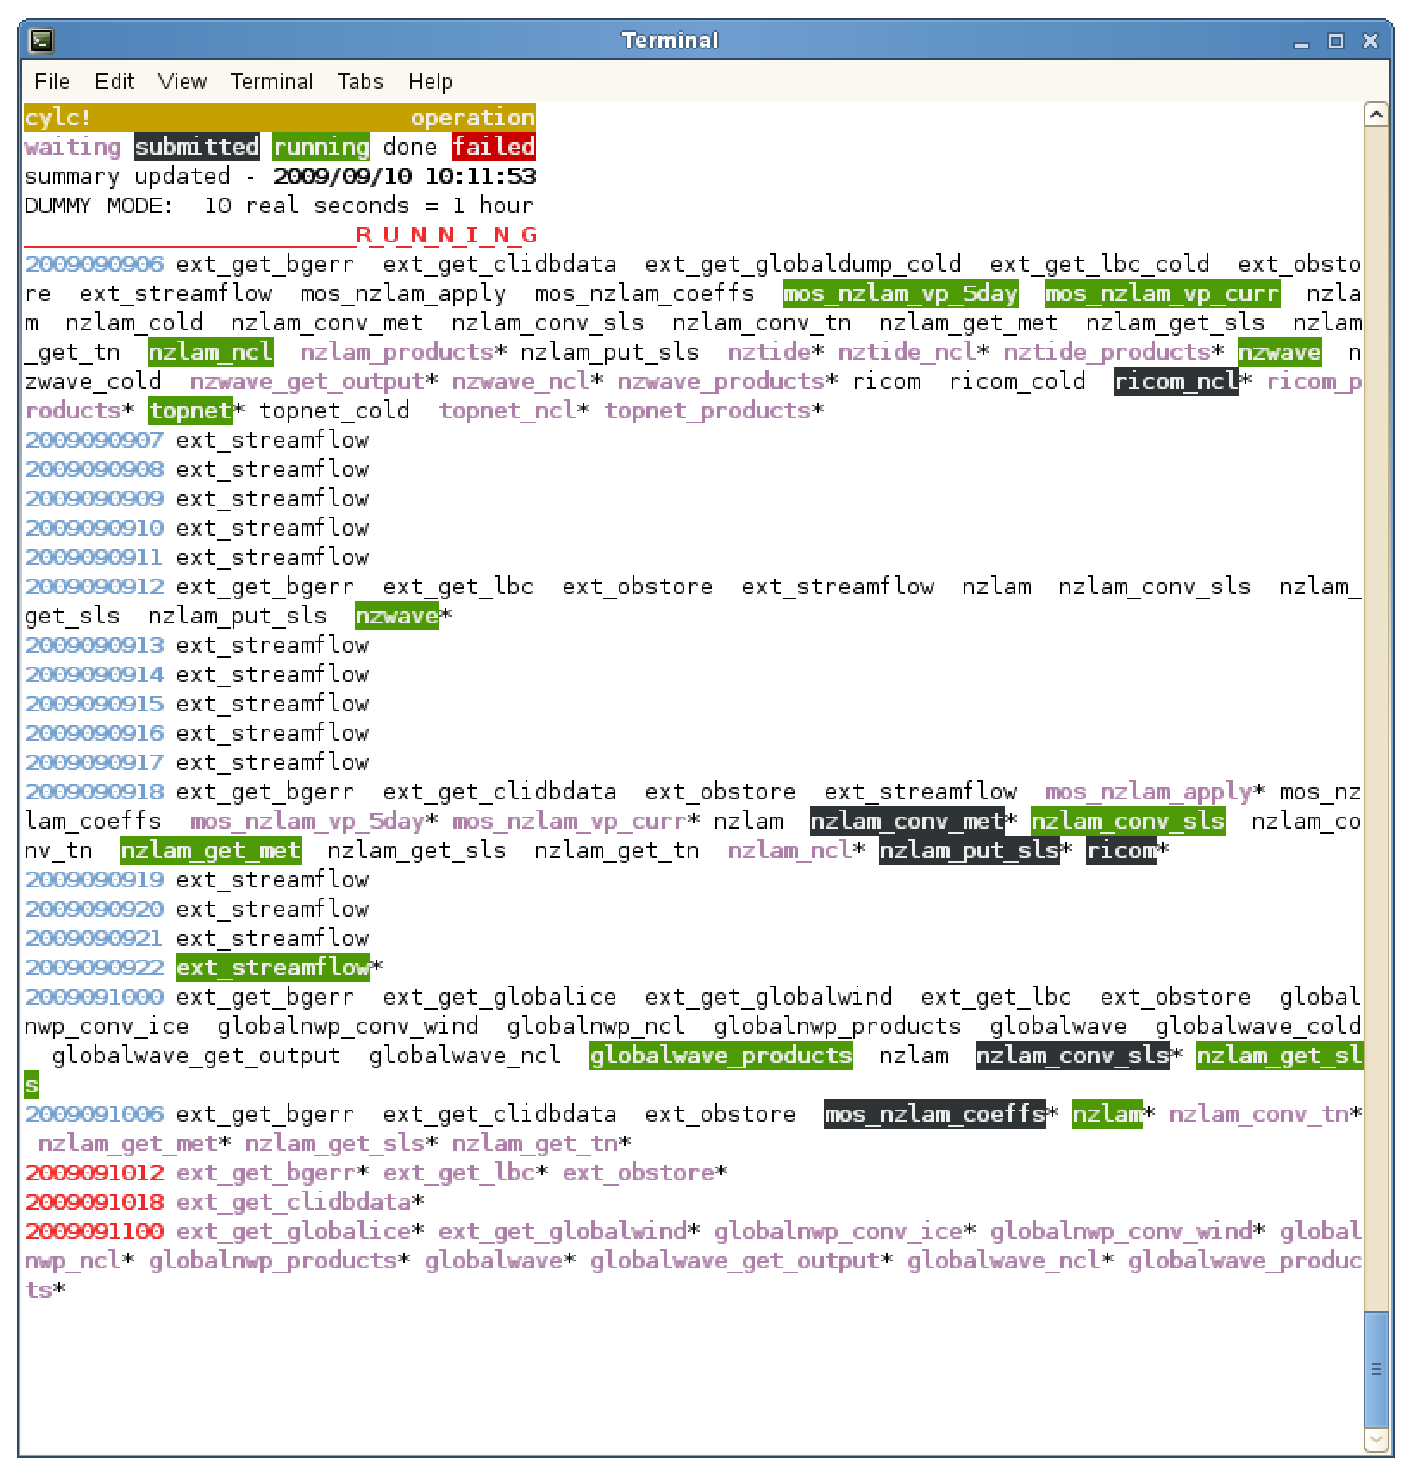
\includegraphics[width=14cm]{eco-monitor} 
    \end{center}
    \caption[monitor view of EcoConnect]{\small The main terminal-based
    cylc system monitor viewing the entire EcoConnect system.}
\end{figure} 

Figure~\ref{fig-monitor-eco} shows the standard monitor view of the
entire ecoconnect operation.

\pagebreak
\section{A Complete Working Example}
\label{ACompleteWorkingExample}

This section contains complete taskdef file and task script listings,
from \lstinline= [CYLC_DIR]/system/userguide/= , that implement the
example used to illustrate the forecast systems scheduling discussion in
{\em How Cylc Works} (Section~\ref{HowCylcWorks}).  While this is
clearly not a real forecasting system, it does have the properties of a
real system as far as scheduling is concerned.  


%THIS FILE IS INCLUDED AUTOMATICALLY IN THE USERGUIDE LaTeX SOURCE
%DURING DOCUMENT PROCESSING

This example system can be run in real and dummy modes; the result
(scheduling wise) should be essentially identical. The task scripts
invoked in real mode create zero-sized output files with the
\lstinline=touch= command, and input files are ``read'' by simply
detecting the file's existence.  All tasks read and write files from a
common location, to simplify the system for illustrative purposes. See
{\em Handling Real Dependencies}
(Section~\ref{HandlingRealDependencies}) for how to manage input and
output files in a more realistic system. 

The Unix 'sleep' command is used to get the trivial example tasks to
execute in the right amount of time (as defined in their taskdef files),
but scaled by \lstinline=$REAL_TIME_ACCEL=, an environment variable
defined in the system config module, so that the system runs quickly 
even in real mode.

The system contains the following tasks:

\begin{itemize}
    \item {\bf A} - could be an atmospheric forecast model,
    it depends on external real time obs and its own restart file.
    \item {\bf B} - could be a sea state model, it depends on 
    outputs generated by A, and its own restart file.
    \item {\bf C} - could be a storm surge model, it depends on 
    outputs generated by A, and its own restart file.
    \item {\bf D} - post processes outputs generated by B and C.
    \item {\bf E} - post processes outputs generated by B.
    \item {\bf F} - post processes outputs generated by C.
    \item {\bf X} - a {\em contact task} that gets the obs data required
    by A, at 1 hour past its reference time. X has no prerequisites and
    therefore runs immediately its contact time has passed.
\end{itemize}

There are also two additional tasks not mentioned in Section~\ref{HowCylcWorks}:

\begin{itemize}
    \item {\bf startup} - a oneoff task that cleans out the system
    workspace (used by all tasks for their output files, in this
    example) at startup.
    \item {\bf coldstart} - a oneoff task provides the initial restart
    prerequisites required by the forecast models (once the system
    is cycling these are provided by previous forecasts). 
\end{itemize}

Task F illustrates the use of cylc's {\em task wrapping} mechanism
(Section~\ref{TaskWrapping}) for running unmodified external tasks. 
The taskdef file ENVIRONMENT key is used to put the cycle time
into the task execution environment in the form expected by the wrapped
external task (\lstinline=$ANALYSIS_TIME= in this case). 

The \lstinline=$NEXT_CYCLE_TIME= and \lstinline=$NEXT_NEXT_CYCLE_TIME=
variables defined in the task definition files, and read by the external
``forecast model'' scripts, are just a convenience to allow the
minimalist external tasks to avoid doing their own cycle time arithmetic
to compute the validity times of their restart outputs.

To run the example system follow the {\em Quick Start Guide}
(Section~\ref{QuickStartGuide}) from the `configure' step onward. Be
careful to set an initial cycle time in the past, or else nothing will
happen until until the start time is reached.

To understand what happens when the system starts up (why, for instance,
a lot of {\em X}'s all go off at once) see {\em System Startup}
(Section~\ref{SystemStartup}).



\lstset{ basicstyle=\color{basic}\scriptsize\ttfamily }

\pagebreak
\input{example-system.tex}

\section{Other Working Examples}
\label{OtherWorkingExamples}

\subsection{Nested}

In this working example system, {\em task C} from the userguide system
has been replaced by a {\em userguide task} which is itself an entire
sub-system running under its own scheduler.

If you run this, configure and register both the userguide and nested
systems. Then start two system monitors, one to follow each system,
before starting the scheduler on the nested system. You should see that 
whenever a new `userguide' task runs in the nested system, a separate
instance of the entire userguide example system will start up and run
for a single cycle. When the subsystem finishes and exits, the
corresponding task in the main system will drop into the finished state.

This example is included because it rather nicely illustrates the power
and flexibility of cylc. That said, the author cannot think of any good
reason why you would actually want to do this in a real forecasting
system! It would almost certainly be better to include the sub-system
tasks in the main system.

\subsection{File-Move}

This working example system illustrates to things:

\begin{itemize}
    \item How you can move real input/output files around to connect
        tasks at the control system level, rather than expecting the
        external tasks themselves to know about the wider system (i.e.\
        where to get input files that are generated by another task).
        See {\em Handling Real Dependencies}
        (Section~\ref{HandlingRealDependencies} for more on this.

    \item How to invoke a generic task script, that can potentially
        implement many system tasks, with task-specific inputs supplied
        via the execution environment specified in taskdef files.

\end{itemize}

\subsection{Distributed}

This working example is a variant of the file-move example system in
which one of the tasks executes on another machine on the network. The
{\em file-transfer} task script is invoked twice, once the `put' task,
which puts input files on the remote machine, and once for the `get'
task, which retrieves outputs from the remote machine once the remote
task has finished.

This example system serves to illustrate two things:

\begin{itemize}
    \item that cylc can control tasks distributed across the network.
    \item that cylc can use different job submission methods for
        different tasks.
\end{itemize}

Unlike the other example systems, this one will not work ``out of the
box''. You will to have passwordless ssh configured to the remote
machine, install the remote task script on it, and specify the right
hostname in the taskdef file.


\pagebreak
\subsection{SCS Demo}

This example system, which resides in 
\lstinline=$CYLC_DIR/systems/scs-demo=,
demonstrates how to set up a single Met Office
UM-based forecast analysis suite that would normally be run by SCS.
Features that distinguish this system are:

\begin{itemize}

    \item dummy mode only - no tasks scripts have been implemented.

    \item restricted start time (see the system config file) - the
        system can cold start at 06Z only

    \item not all tasks run in all cycles - see arch, g\_lbc, post2

    \item intercycle dependence other than forecast model restart 
        dependencies - g_lbc outputs are used by two subsequent UM_nz
        tasks.

    \item UM\_nz behaves differently in different cycles - 00,12Z short
        forecast, 06,18Z long forecast.

    \item the VAR task depends on the OPS tasks {\em completing} - i.e.\
        succeeding OR failing, because obs processing is expected to
        fail sometimes.  Try this with:

        \begin{lstlisting}
cylc start -d --fail-out=OPS1%YYYYMMDDHH ...
        \end{lstlisting}

        VAR will not be delayed, but the failed OPS task does have to be
        killed or it will eventually stall the system at the maximum
        runahead time (see {\em System Config Files},
        Section~\ref{SystemConfigFiles}).
        
\end{itemize}

Here's some more information from the system README file:

\lstset{language=}
\lstinputlisting{../systems/scs-demo/README.txt}

\subsubsection{Finishing It Off}

Cylc needs to be able to invoke each system task by calling a named
script (which can in turn invoke other scripts, of course) that takes
its cycle time from the environment as  \lstinline=$CYCLE_TIME=.

Configure the OPS, VAR, and UM tasks as standalone jobs via their
respective UIs. Some minor surgery might be required on the resulting
job scripts to get the desired result.  Add cylc messaging to report
startup, finish, failure, and completed outputs.

\pagebreak
\section{Command Reference}
\label{CommandReference}

This section of the userguide is auto-generated from the current
self-documenting command set during document processing; additional
notes are appended after some commands.

\lstset{ basicstyle=\color{basic}\footnotesize\ttfamily }
\lstset{language=usage}

\input{commands.tex}

\section{Master Task Definition Template}
\label{MasterTaskDefinitionTemplate}

Listed below is the full task definitition template with all items
documented.

\lstset{language=cylctaskdef}

\lstinputlisting{../templates/taskdef/master.def}

\lstset{language=}

\pagebreak
\subsection{More Complex Task Behaviour}
labelsubsection{MoreComplexTaskBehaviour}

DETAIL WHEN IS IT NECESSARY TO DERIVE PYTHON TASK CLASSES DIRECTLY
I.E.\ WHEN ARE CYLC TASK DEFINITION FILES NOT SUFFICIENT.
(In EcoConnect: only streamflow and topnet)

\pagebreak
\section{Master Task Script Templates}
\label{MasterTaskScriptTemplates}


See also {\em Task Wrapping} (Section~\ref{TaskWrapping}), which allows
cylc to control unmodified external tasks (i.e.\ you don't need to 
use the task scripts described in this section).

\lstset{language=bash}

The following variables are automatically exported by cylc into
the execution environment of a each task:
\begin{itemize}
   \item \lstinline=$SYSTEM_NAME= - registered name of the running system.
   \item \lstinline=$TASK_NAME= - how cylc refers to the task (not the
       filename of the task script). 
   \item \lstinline=$CYCLE_TIME= - task-specific forecast cycle time.
   \item \lstinline=$CYLC_NS_GROUP= - Pyro nameserver group name used by the system.
   \item \lstinline=$CYLC_NS_HOST= - Pyro nameserver hostname.
\end{itemize}

\lstset{language=bash}
When called by a task script, \lstinline=cylc message= read the task
name and cycle time from the environment and uses these to target the
correct task proxy object within the running scheduler.
\lstset{language=cylctaskdef=}
A task can also access any task-specific
environment variables set in the task definition file
\lstinline=ENVIRONMENT= key.

\lstset{language=bash}

If a task script is executed manually or by \lstinline=cylc run-task=
then \lstinline=cylc message= will print to stdout instead of attempting
to communicate with a task proxy object registered in a Pyro nameserver.


\lstset{language=bash}

\pagebreak
\subsection{Free Tasks}
\lstinputlisting{../templates/scripts/free-task.sh}

\pagebreak
\subsection{Tied Tasks}
\lstinputlisting{../templates/scripts/tied-task.sh}

\appendix

\pagebreak
\section{Object Oriented Programming}
\label{ObjectOrientedProgramming}

Cylc relies heavily on Object Oriented Programming (OOP) concepts,
particularly the {\em polymorphic} nature of the task proxy objects.
This section gives a very minimal explanation of what this means;
please refer to an OOP reference for more detail.

A {\bf class} is a generalisation of data type to include behaviour
(i.e.\ functions or methods) as well as state. 

%For example, a $shape$ class could define a $position$ data member to
%hold the location of a shape object, a $move()$ method that by which
%a shape object can alter its position, and a $draw()$ method that
%causes it to display itself on screen.

An {\bf object} is a more or less self contained specific instance
of a class. This is analagous to specific integer variables being 
instances of the integer data type.

A {\bf derived class} or {\bf subclass} {\em inherits} the properties
(methods and data members) of its parent class. It can also override
specific properties, or add new properties that aren't present in the
parent. Calling a particular method on an object invokes the object's
own method if one is defined, otherwise the parent class is searched,
and so on down to the root of the inheritance graph. 

%For example, we could derive a $circle$ class from $shape$, adding a
%`radius' data member and overriding the $draw()$ to get circle objects
%to display themselves as actual circles.  Because we didn't override the
%$move()$ method, calling $circle.move()$ would invoke the base class
%method, $shape.move()$. 


{\bf Polymorphism} is the ability of one type to appear as and be used
like another type.  In OOP languages with inheritance, this usually
refers to the ability to treat derived/sub-class objects as if they were
members of a common base class. In particular, a group of mixed-type
objects can all be treated as members of a common base class. 
%For example, a group of %$circles$, $triangles$, and $squares$ could 
%be manipulated by code designed entirely to handel $shapes$; calling
%$[shape].draw()$ will invoke the right derived class $draw()$ method. 
This is a powerful mechanism because it allows an existing program,
without modification, to manipulate new objects so long as they 
derive from the same base class as the original objects.
%If we later derive an entirely new kind of shape ($hexagon$, say) with
%it's own unique behaviour, the existing program, without modification,
%will process the new objects in the proper hexagon-specific way.  

In cylc, all task proxy objects are derived from a base class that 
embodies the properties and behaviour common to all task proxies. 
The scheduling algorithm works with instances of the base class so that
any current or future derived task object can be handled by the program
without modification (other than deriving the new subclass itself).


\pagebreak
\section{Pyro} 
\label{Pyro}

Pyro (Python Remote Objects) is a widely used open source objected
oriented Remote Procedure Call technology, see {\em
http://pyro.sourceforge.net}.

\subsection{Pyro Software License (MIT license)}
\label{PyroSoftwareLicense(MITlicense)}

Pyro is Copyright (c) 2002  by Irmen de Jong.

Permission is hereby granted, free of charge, to any person obtaining a
copy of this software and associated documentation files (the
``Software''), to deal in the Software without restriction, including
without limitation the rights to use, copy, modify, merge, publish,
distribute, sublicense, and/or sell copies of the Software, and to
permit persons to whom the Software is furnished to do so, subject to
the following conditions:

The above copyright notice and this permission notice shall be included
in all copies or substantial portions of the Software.

THE SOFTWARE IS PROVIDED ``AS IS'', WITHOUT WARRANTY OF ANY KIND,
EXPRESS OR IMPLIED, INCLUDING BUT NOT LIMITED TO THE WARRANTIES OF
MERCHANTABILITY, FITNESS FOR A PARTICULAR PURPOSE AND NONINFRINGEMENT.
IN NO EVENT SHALL THE AUTHORS OR COPYRIGHT HOLDERS BE LIABLE FOR ANY
CLAIM, DAMAGES OR OTHER LIABILITY, WHETHER IN AN ACTION OF CONTRACT,
TORT OR OTHERWISE, ARISING FROM, OUT OF OR IN CONNECTION WITH THE
SOFTWARE OR THE USE OR OTHER DEALINGS IN THE SOFTWARE.
                                          
\subsection{Single- or Multi-Threaded Pyro?}
\label{Single-orMulti-ThreadedPyro?}

In single threaded mode Pyro's \lstinline=handleRequests()= returns
after either a timeout has occurred or at least one request
(i.e.\ remote method call) was handled. Using \lstinline|timeout = None| 
allows us to process tasks {\em only} after remote method invocations
come in.  Further, we can detect the remote calls that actually change
task states, and thereby drop into the task processing code only when
necessary, which eliminates a lot of extraneous output when debugging
the task processing loop (e.g.\ in dummy mode there are a lot of remote
calls on the dummy clock object, which does not alter tasks at all). 

In multithreaded mode, \lstinline=handleRequests()= returns immediately
after creating a new request handling thread for a single remote object,
and thereafter remote method calls on that object come in asynchronously
in the dedicated thread. This is not good for cylc's scheduling
algorithm because tasks are only set running in the task processing
block which can be delayed while \lstinline=handleRequests()= blocks waiting
for a new connection to be established, even as messages that warrant
task processing are coming in on existing connections. The only way
around this seems to be to do task processing on \lstinline=handleRequests()=
timeouts which results in a lot of unnecessary processing when nothing
important is happening.

\subsection{Running Pyro}
\label{RunningPyro}

To see if there is a Pyro nameserver running already on your network
segment, use \lstinline=pyro-nsc [-h host] [-p port] ping=. Invoke the
command without arguments to see a list of options.

\lstset{language=bash}

\begin{lstlisting}
$ pyro-nsc ping
Locator: searching Pyro Name Server...
Locator: retry 1
Locator: searching Pyro Name Server...
Locator: retry 1
Trying host oliverh-33191VL
Locator: contacting Pyro Name Server...
NS is at 127.0.0.2 (oliverh-33191VL.greta.niwa.co.nz) port 9090
NS is up and running!

$ pyro-nsc -h localhost ping
Locator: contacting Pyro Name Server...
NS is at 127.0.0.1 (localhost) port 9090
NS is up and running!
\end{lstlisting}

To start a Pyro nameserver, use \lstinline{nohup} so that it
will not die with your terminal session: 

\begin{lstlisting}
 nohup pyro-ns &
\end{lstlisting}

For more information, see the Pyro userguide.

\pagebreak
\section{Miscellaneous Notes}
\label{MiscellaneousNotes}

\subsection{Cycle Dependent Prerequisites}

It may be better to split a task into two (or more) than use this 
capability.

\subsection{Orderly Product Generation}
\label{OrderlyProductGeneration}

Note that ``correct scheduling'' is not equivalent to ``orderly
generation of products by cycle time'' - under cylc a product
generation task will trigger as soon as its prerequisites are satisfied,
whether or not other tasks associated with the same cycle time are
running yet. If your product presentation or delivery system demands
that all products for one cycle are complete before any from the next
cycle, then (a) this is inefficient - fix it!, or (b) introduce artificial
dependencies into your system to enforce strict sequential cycling (but
that, of course, nullifies the principal advantage of using cylc in the
first place!), or (c) write a script that monitors the output from 
your cylc system and reports completion of a cycle only when the last
products associated with that cycle are complete. 

%\subsection{Catching Up}
%labelsubsection{CatchingUp}
%
%The state of being ``caught up'' or not is a property of individual
%tasks, not the whole system, and additionally it should only matter to
%external contact tasks, i.e.\ those that wait on external data that is
%available at a wall clock time of T (task cycle time) + o (some offset
%insterval). Where this matters an external task can detect whether or
%not it has caught up (and signal this to its proxy object in cylc) by
%comparing its cycle time (and offset) to the wall clock time.

\subsection{Running Multiple Instances Of The Same System}
\label{RunningMultipleInstancesOfTheSameSystem}

What this means: the exact same task class and config modules, under
different registered names, AND the same task scripts (under scripts/)
- although the registered name could be used in all important
directories at run time, potentially to access a different set of 
executables\dots

Consequences - dummy mode fine (e.g.\ multiple users running the standard
cylc example systems)

             - real mode: the external tasks must not interfere! Could
             use system name in all important dir paths, but prob better 
             to copy the system def directory AND invoke different versions
             of the external tasks (e.g.\ under /oper and /test)

    Registered names are also used along with your username to construct
    a unique Pyro nameserver `group name' for any system that you run.
    This allows multiple systems, from multiple users, to run at once
    without interfering with each other (i.e.\ external tasks will not
    be able to send messages to the wrong scheduler instance).
    
    You can register the same system under multiple names. This makes it
    is possible, in principle, to run multiple instances of the same
    system at once. Be aware, however, that the external system must
    also be capable of doing this (perhaps by incorporating the cylc
    system name into its input and output directory paths and so on - it
    may be safer to run multiple *copies* of a system, each with
    different configuration, task definitions, and scripts, so that the
    external systems are in effect separate).

    However: registered system name is available for use in global 
    env vars via sytem config module, AND from task-specific 
    environment in taskdef files, via \lstinline=$SYSTEM_NAME=.

\subsection{How Cylc Interacts With Batch Queue Schedulers}
\label{HowCylcInteractsWithBatchQueueSchedulers}

Cylc dynamically adapts to any external execution environment. It just
decides when a task is *ready* to run - i.e.\ when its prerequisites 
are satisfied.  If the external task is delayed because of resource
contention, it will not report its outputs complete until it does run.

\subsection{Known Bugs and Limitations}

\begin{itemize}
    \item cycle time minimum granularity = 1 hour. Note this is
        only loosely connected to when, or how frequently, a task
        actually runs, and only in real time operation. Would be easy to
        extend to minutes and seconds, if necessary.

    \item it is assumed that every task runs at least once in 24 hours
        (see the taskdef CYCLES key). It would be easy to extend this to
        less frequent tasks, if required.

    \item why we need the nudge option - maybe should use a timeout too.

\end{itemize}

\subsection{Upgrading Taskdefs}

Suggested easy way to make textual changes to many taskdef files en
masse (e.g.\ to make them compatible with a new version of cylc):

\begin{itemize}
    \item record all pending changes to the system repository
    \item make bulk changes in-place using perl's powerful regex 
       substitution mechanism, e.g.:
       \begin{lstlisting}
$ for F in *.def; do perl -pi -e 's/OLD/NEW/g' $F; done
       \end{lstlisting}
   \item check this had the desired effect with 
       \lstinline=darcs whatsnew=. If not, revert and try again.
\end{itemize}


\section{Safety Netting}
\label{SafetyNetting}

\begin{itemize}
    \item dummy mode: get scheduling right before running real tasks
    \item automatic state dump prior to system interventions - restart
        from prior state if necessary.
    \item practice mode: instantly clone an accelerated dummy mode copy
        of you operational system in its current running state (or its
        most recent state prior to shutdown) current state) and use it
        to try out system interventions as many times as you like
        necessary without affecting the state of the operational system.
\end{itemize}

\section{Failure Recovery Scenarios}
\label{Failure Recovery Scenarios}

\begin{itemize}
    \item {\em One forecast cycle runs into the next, after a delay in
        operations}. This is no problem for cylc; every task runs as
        soon as it can run, regardless of forecast cycle.

    \item {\em A delayed parallel trial or case study catches up to real
        time operation}. This is no problem for cylc; as explained in
        Section~\ref{foo} any cycl system will seamlessly transition in
        and out of ``normal real time operation'' (distinct cycles
        triggered by the wall clock) as needed.

    \item {\em An external task fails, but can be fixed}. For example, a
        forecast model aborts trying to read a corrupted data file that
        can be regenerated correctly. The failed task will be noted by
        cylc, and its downstream dependants will not be able to run,
        but other tasks will carry on as normal while you address the
        problem. When fixed, use `cylc reset' to get the failed task to
        run again, after which it and its downstream dependants will
        catch up to the rest of the system as quickly as possible.

    \item {\em An important external task fails, but cannot be fixed.}
        In this case, if the task has a lot of downstream dependants,
        you will presumably need omit one or more cycles of the affected
        tasks, and cold start their part of the system at a the earliest
        possible subsequent cycle.  To do this, insert the relevant cold
        start task, or task group, at the later cycle, then purge the
        failed task and everything that depends on it (and on them, and
        so on) down to the cold start time.  Other parts of the system 
        not directly affected should be able to carry on over the hole
        so long as the forecast models involved write out sufficient 
        restart outputs to do so.

    \item {\em HELP, I screwed up a system intervention} such as the
        above!  Before any operation that alters the sytem state, cycl
        automatically dumps state and reports the state dump filename in
        the main log.  Shut the system down and restart it from the
        pre-screwup state. Then retry your intervention in practice mode
        before doing it for real!

\end{itemize}


\end{document}
